\documentclass[aspectratio=169]{beamer}

\usepackage[T5]{fontenc}
\usepackage[utf8]{inputenc}
\usepackage{lmodern}

\usetheme{Madrid}

\usepackage{graphicx}
\usepackage{multicol}
\usepackage{amsmath,amssymb}

% Outline look: blue text, numbered, no balls
\setbeamertemplate{section in toc}{%
  \leavevmode\inserttocsectionnumber.~\inserttocsection\par}
\setbeamercolor{section in toc}{fg=blue}

\hypersetup{colorlinks=true, urlcolor=blue}

\newcommand{\backbtn}{%
  \hfill\hyperlink{outline}{\beamerbutton{Mục lục}}}


% Giảm khoảng cách trên/dưới công thức hiển thị để slide gọn hơn
\makeatletter
\def\tight@disp{\setlength\abovedisplayskip{4pt plus 2pt}%
  \setlength\belowdisplayskip{4pt plus 2pt}%
  \setlength\abovedisplayshortskip{2pt plus 1pt}%
  \setlength\belowdisplayshortskip{2pt plus 1pt}}
\g@addto@macro\normalsize{\tight@disp}
\g@addto@macro\small{\tight@disp}
\g@addto@macro\footnotesize{\tight@disp}
\g@addto@macro\scriptsize{\tight@disp}
\makeatother

\title[Phương pháp năng lượng]{Phương pháp năng lượng}
\author[© N. V. Sỹ]{Nguyễn Văn Sỹ}
\institute[TNUT]{%
  Bộ môn Hệ thống Công nghiệp \\
  Trường Đại học Kỹ thuật Công nghiệp \\
  \href{mailto:vansy@tnut.edu.vn}{vansy@tnut.edu.vn}}
\date[Cơ học vật liệu]{\large Cơ học vật liệu – Phương pháp năng lượng \\[0.5em] \footnotesize \copyright\ Nguyễn Văn Sỹ}

\begin{document}

\begin{frame}
  \titlepage
\end{frame}
%====================
\begin{frame}{Tài liệu tham khảo}
	\small
	F. P. Beer, E. R. Johnston, Jr., J. T. DeWolf, D. F. Mazurek,
	\emph{Mechanics of Materials}, 6th ed., McGraw-Hill, New York, 2012.
	
	\vspace{1em}
	\footnotesize\color{gray}
	Toàn bộ hình vẽ trong bài giảng được trích từ giáo trình trên, chỉ sử dụng
	cho mục đích giảng dạy nội bộ.
\end{frame}
% ===== OUTLINE SLIDE =====
\begin{frame}[t]{Nội dung}
  \hypertarget{outline}{}
  \tiny
  \begin{multicols}{2}
    \tableofcontents[hideallsubsections]
  \end{multicols}
\end{frame}

% ===== CONTENT SLIDES =====
\section{Năng lượng biến dạng}
\begin{frame}[t]{Năng lượng biến dạng}
  \begin{columns}[T]
    \column{0.58\textwidth}
      \small
      \begin{itemize}
        \setlength{\itemsep}{0.4em}
        \item Một thanh đồng chất chịu tải trọng tăng dần chậm.
        \item Công phân tố do tải trọng $P$ thực hiện khi thanh giãn dài thêm
              một đoạn nhỏ $dx$:
        \[
          dU = P\,dx = \text{công phân tố}
        \]
        bằng diện tích dải rộng $dx$ dưới biểu đồ tải trọng -- biến dạng.
        \item Tổng công do tải trọng thực hiện ứng với biến dạng $x_1$:
        \[
          U = \int_0^{x_1}P\,dx = \text{tổng công} = \text{năng lượng biến dạng}
        \]
        \item Trường hợp biến dạng đàn hồi tuyến tính:
        \[
          U = \int_0^{x_1}kx\,dx = \tfrac{1}{2}kx_1^2 = \tfrac{1}{2}P_1x_1
        \]
      \end{itemize}
    \column{0.40\textwidth}
      \centering
      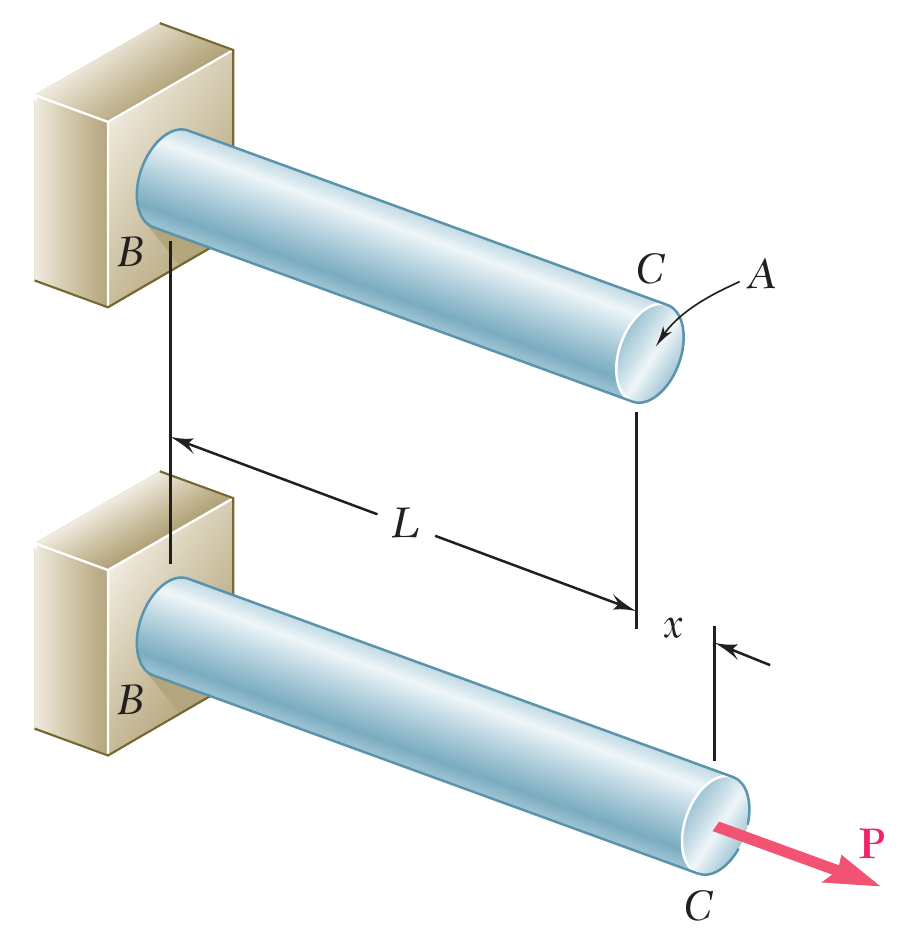
\includegraphics[width=\linewidth,height=1.9cm,keepaspectratio]{Chap_11/fig_11_1.png}\\[2pt]
      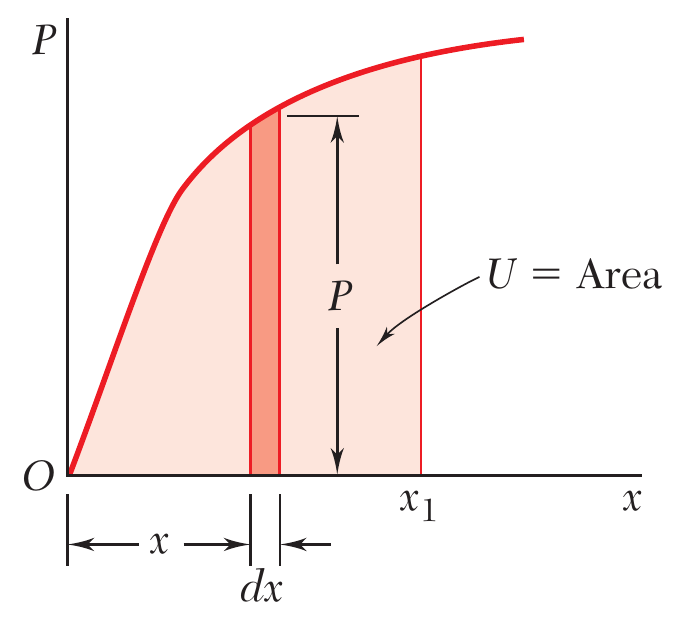
\includegraphics[width=\linewidth,height=1.9cm,keepaspectratio]{Chap_11/fig_11_3.png}\\[2pt]
      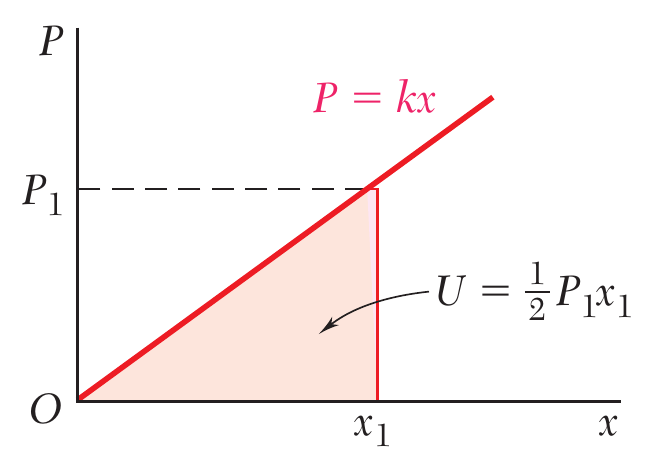
\includegraphics[width=\linewidth,height=1.9cm,keepaspectratio]{Chap_11/fig_11_4.png}
  \end{columns}
\end{frame}
% ===========
\section{Mật độ năng lượng biến dạng}
\begin{frame}[t]{Mật độ năng lượng biến dạng}
  \begin{columns}[T]
    \column{0.58\textwidth}
      \small
      \begin{itemize}
        \setlength{\itemsep}{0.5em}
        \item Để loại bỏ ảnh hưởng của kích thước, tính năng lượng biến dạng
              trên một đơn vị thể tích:
        \[
          \frac{U}{V} = \int_0^{x_1}\frac{P}{A}\frac{dx}{L}
        \]
        \[
          u = \int_0^{\varepsilon_1}\sigma_x\,d\varepsilon_x
            = \text{mật độ năng lượng biến dạng}
        \]
        \item Tổng mật độ năng lượng biến dạng do biến dạng gây ra bằng diện
              tích dưới đường cong đến $\varepsilon_1$.
        \item Khi dỡ tải, ứng suất trở về không nhưng còn lại biến dạng dư.
              Chỉ phần năng lượng biến dạng ứng với diện tích tam giác được hoàn
              trả.
        \item Phần năng lượng còn lại tiêu hao để làm biến dạng vật liệu được
              tỏa ra dưới dạng nhiệt.
      \end{itemize}
    \column{0.40\textwidth}
      \centering
      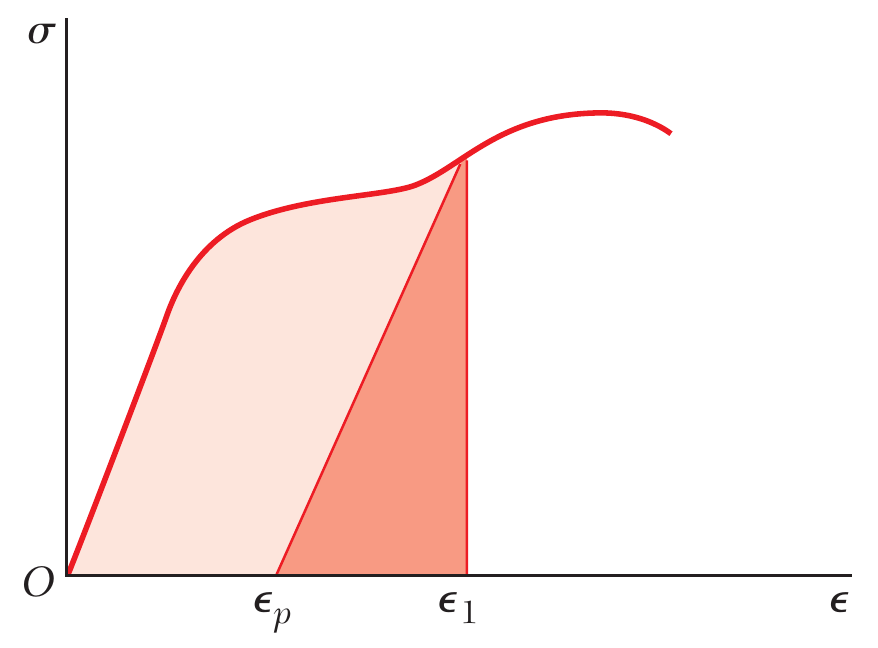
\includegraphics[width=\linewidth,height=5.5cm,keepaspectratio]{Chap_11/fig_11_6.png}
  \end{columns}
\end{frame}
% ===========
\begin{frame}[t]{Mật độ năng lượng biến dạng (tiếp)}
  \begin{columns}[T]
    \column{0.58\textwidth}
      \small
      \begin{itemize}
        \setlength{\itemsep}{0.5em}
        \item Mật độ năng lượng biến dạng ứng với $\varepsilon_1 = \varepsilon_R$
              là \emph{mô đun dai} (modulus of toughness).
        \item Năng lượng trên một đơn vị thể tích cần thiết để làm vật liệu bị
              phá hủy liên quan đến độ dẻo cũng như giới hạn bền của vật liệu.
        \item Nếu ứng suất nằm trong giới hạn tỉ lệ:
        \[
          u = \int_0^{\varepsilon_1}E\varepsilon_x\,d\varepsilon_x
            = \frac{E\varepsilon_1^2}{2} = \frac{\sigma_1^2}{2E}
        \]
        \item Mật độ năng lượng biến dạng ứng với $\sigma_1 = \sigma_Y$ là
              \emph{mô đun đàn hồi tích lũy} (modulus of resilience):
        \[
          u_Y = \frac{\sigma_Y^2}{2E} = \text{mô đun đàn hồi tích lũy}
        \]
      \end{itemize}
    \column{0.40\textwidth}
      \centering
      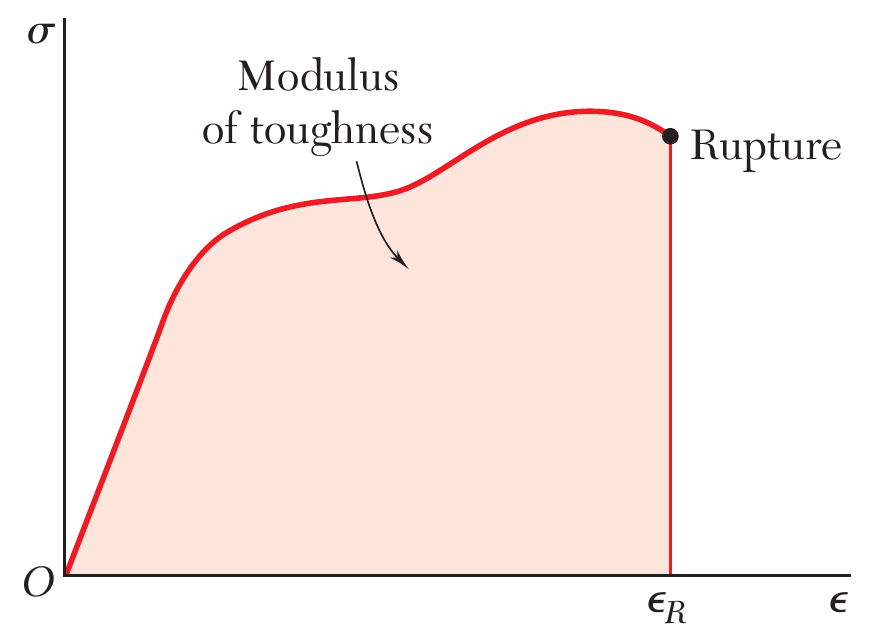
\includegraphics[width=\linewidth,height=2.9cm,keepaspectratio]{Chap_11/fig_11_7.png}\\[2pt]
      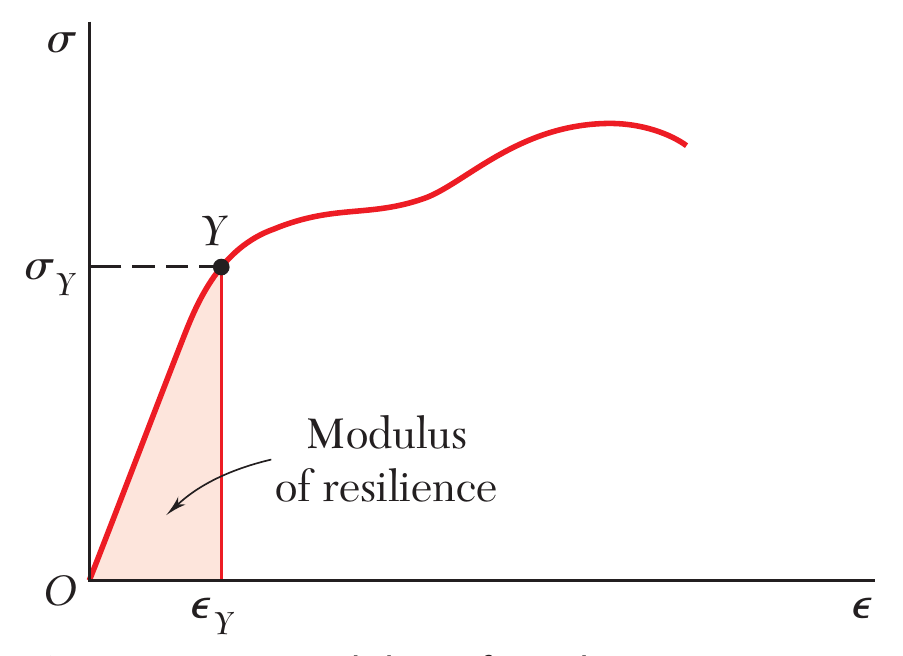
\includegraphics[width=\linewidth,height=2.9cm,keepaspectratio]{Chap_11/fig_11_8.png}
  \end{columns}
\end{frame}
% ===========
\section{Năng lượng biến dạng đàn hồi do ứng suất pháp}
\begin{frame}[t]{Năng lượng biến dạng đàn hồi do ứng suất pháp}
  \begin{columns}[T]
    \column{0.58\textwidth}
      \footnotesize
      \begin{itemize}
        \setlength{\itemsep}{0.20em}
        \item Trong phân tố có phân bố ứng suất không đều:
        \[
          u = \lim_{\Delta V\to0}\frac{\Delta U}{\Delta V} = \frac{dU}{dV}
        \]
        \[
          U = \int u\,dV = \text{tổng năng lượng biến dạng}
        \]
        \item Với $u < u_Y$, tức là dưới giới hạn tỉ lệ:
        \[
          U = \int\frac{\sigma_x^2}{2E}\,dV = \text{năng lượng biến dạng đàn hồi}
        \]
        \item Khi chịu tải trọng dọc trục, $\sigma_x = P/A$, $dV = A\,dx$:
        \[
          U = \int_0^L\frac{P^2}{2AE}\,dx
        \]
        \item Với thanh có mặt cắt ngang không đổi:
        \[
          U = \frac{P^2L}{2AE}
        \]
      \end{itemize}
    \column{0.40\textwidth}
      \centering
      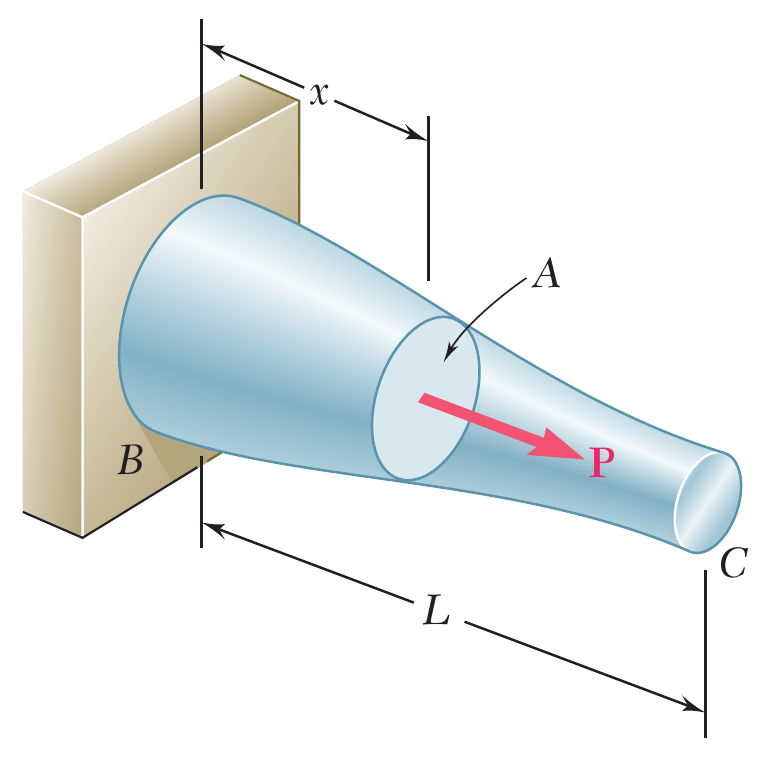
\includegraphics[width=\linewidth,height=2.5cm,keepaspectratio]{Chap_11/fig_11_9.png}\\[2pt]
      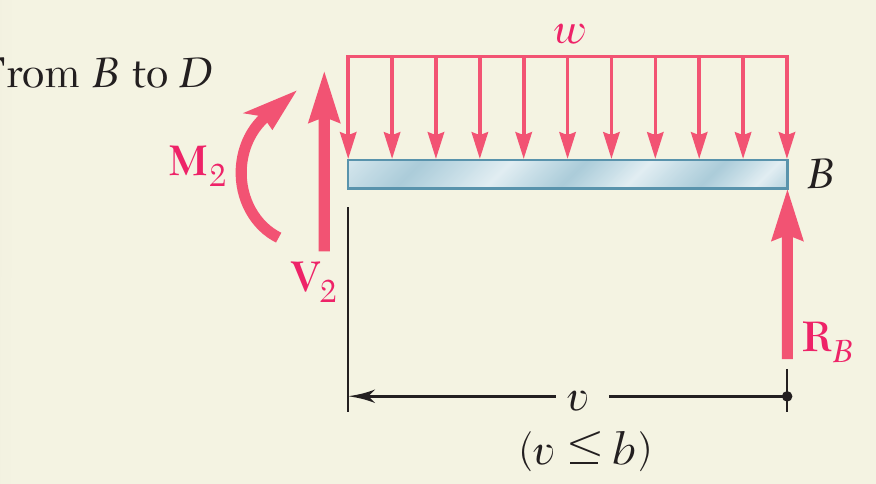
\includegraphics[width=\linewidth,height=2.5cm,keepaspectratio]{Chap_11/sp_11_6_b.png}
  \end{columns}
\end{frame}
% ===========
\begin{frame}[t]{Năng lượng biến dạng đàn hồi do ứng suất pháp (tiếp)}
  \begin{columns}[T]
    \column{0.58\textwidth}
      \small
      \begin{itemize}
        \setlength{\itemsep}{0.4em}
        \item Với dầm chịu uốn:
        \[
          U = \int\frac{\sigma_x^2}{2E}\,dV = \int\frac{M^2y^2}{2EI^2}\,dV
          \qquad \sigma_x = \frac{My}{I}
        \]
        \item Đặt $dV = dA\,dx$:
        \[
          U = \int_0^L\int_A\frac{M^2y^2}{2EI^2}\,dA\,dx
            = \int_0^L\frac{M^2}{2EI^2}\left(\int_Ay^2\,dA\right)dx
        \]
        \[
          U = \int_0^L\frac{M^2}{2EI}\,dx
        \]
        \item Với dầm công xôn chịu lực ở đầu tự do, $M = -Px$:
        \[
          U = \int_0^L\frac{P^2x^2}{2EI}\,dx = \frac{P^2L^3}{6EI}
        \]
      \end{itemize}
    \column{0.40\textwidth}
      \centering
      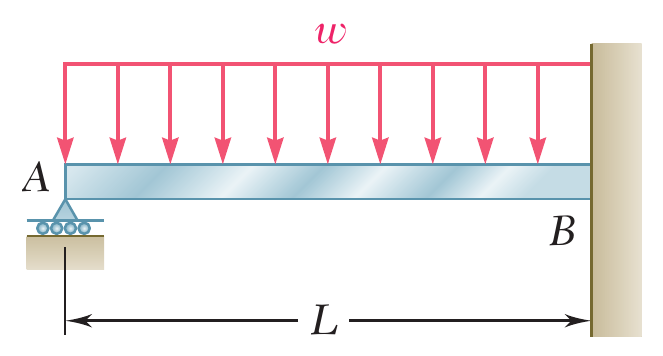
\includegraphics[width=\linewidth,height=2.9cm,keepaspectratio]{Chap_11/fig_11_47.png}\\[2pt]
      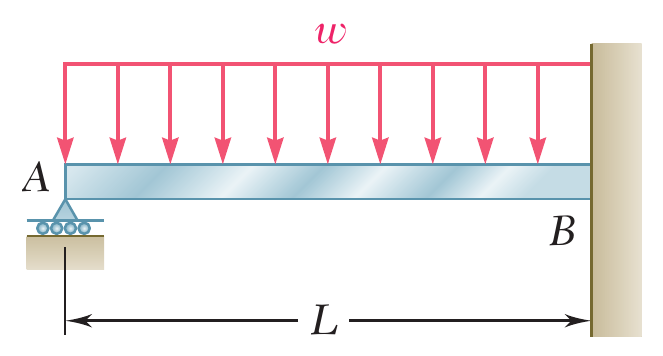
\includegraphics[width=\linewidth,height=2.9cm,keepaspectratio]{Chap_11/fig_11_47.png}
  \end{columns}
\end{frame}
% ===========
\section{Năng lượng biến dạng do ứng suất tiếp}
\begin{frame}[t]{Năng lượng biến dạng do ứng suất tiếp}
  \begin{columns}[T]
    \column{0.58\textwidth}
      \small
      \begin{itemize}
        \setlength{\itemsep}{0.6em}
        \item Với vật liệu chịu ứng suất tiếp trong mặt phẳng:
        \[
          u = \int_0^{\gamma_{xy}}\tau_{xy}\,d\gamma_{xy}
        \]
        \item Với $\tau_{xy}$ trong giới hạn tỉ lệ:
        \[
          u = \tfrac{1}{2}G\gamma_{xy}^2 = \tfrac{1}{2}\tau_{xy}\gamma_{xy}
            = \frac{\tau_{xy}^2}{2G}
        \]
        \item Tổng năng lượng biến dạng được tính từ:
        \[
          U = \int u\,dV = \int\frac{\tau_{xy}^2}{2G}\,dV
        \]
      \end{itemize}
    \column{0.40\textwidth}
      \centering
      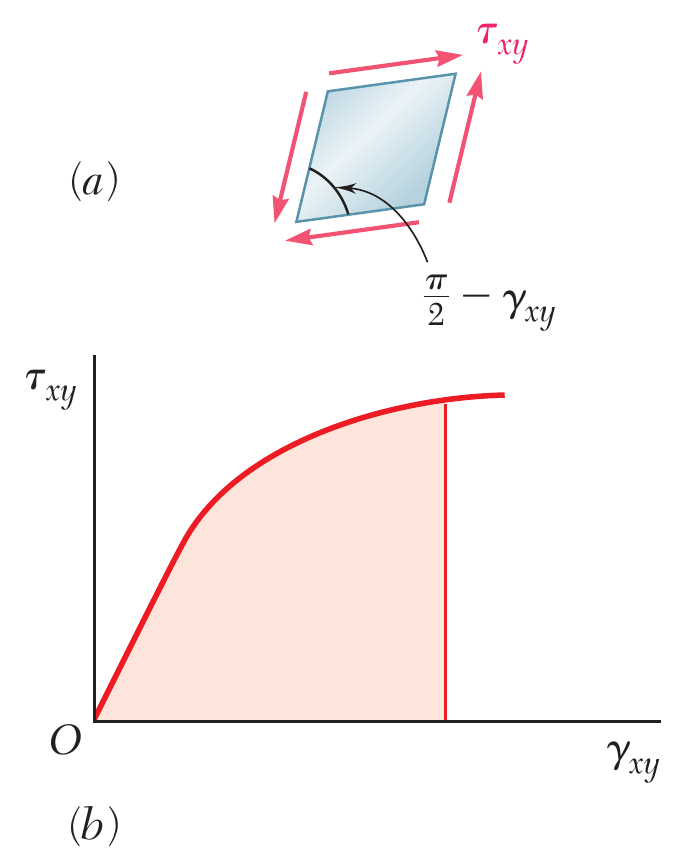
\includegraphics[width=\linewidth,height=5.5cm,keepaspectratio]{Chap_11/fig_11_16.png}
  \end{columns}
\end{frame}
% ===========
\begin{frame}[t]{Năng lượng biến dạng do ứng suất tiếp (tiếp)}
  \begin{columns}[T]
    \column{0.58\textwidth}
      \small
      \begin{itemize}
        \setlength{\itemsep}{0.5em}
        \item Với trục chịu xoắn:
        \[
          U = \int\frac{\tau_{xy}^2}{2G}\,dV = \int\frac{T^2\rho^2}{2GJ^2}\,dV
          \qquad \tau_{xy} = \frac{T\rho}{J}
        \]
        \item Đặt $dV = dA\,dx$:
        \[
          U = \int_0^L\int_A\frac{T^2\rho^2}{2GJ^2}\,dA\,dx
            = \int_0^L\frac{T^2}{2GJ^2}\left(\int_A\rho^2\,dA\right)dx
        \]
        \[
          U = \int_0^L\frac{T^2}{2GJ}\,dx
        \]
        \item Trường hợp trục đồng chất:
        \[
          U = \frac{T^2L}{2GJ}
        \]
      \end{itemize}
    \column{0.40\textwidth}
      \centering
      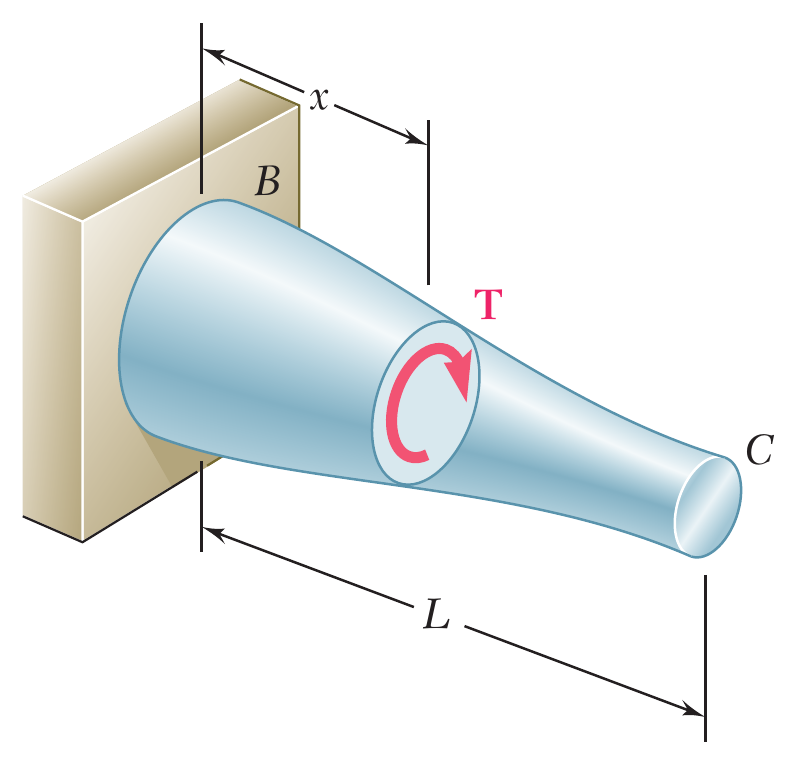
\includegraphics[width=\linewidth,height=2.9cm,keepaspectratio]{Chap_11/fig_11_17.png}\\[2pt]
      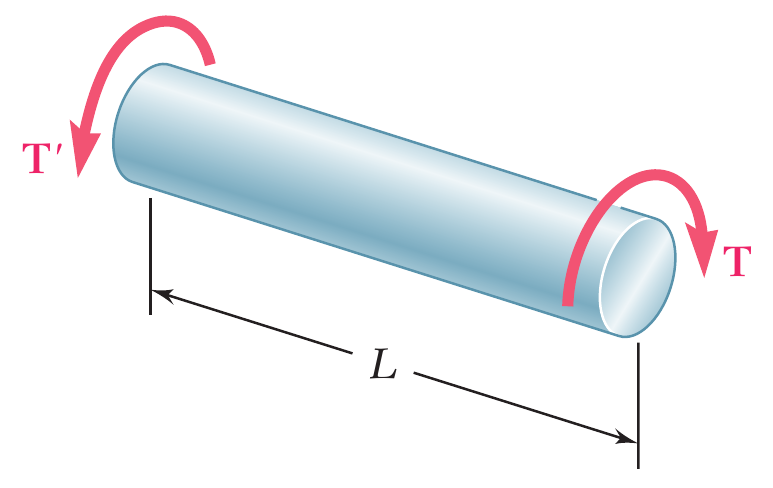
\includegraphics[width=\linewidth,height=2.9cm,keepaspectratio]{Chap_11/fig_11_18.png}
  \end{columns}
\end{frame}
% ===========
\section{Bài mẫu 11.2}
\begin{frame}[t]{Bài mẫu 11.2}
  \begin{columns}[T]
    \column{0.42\textwidth}
      \centering
      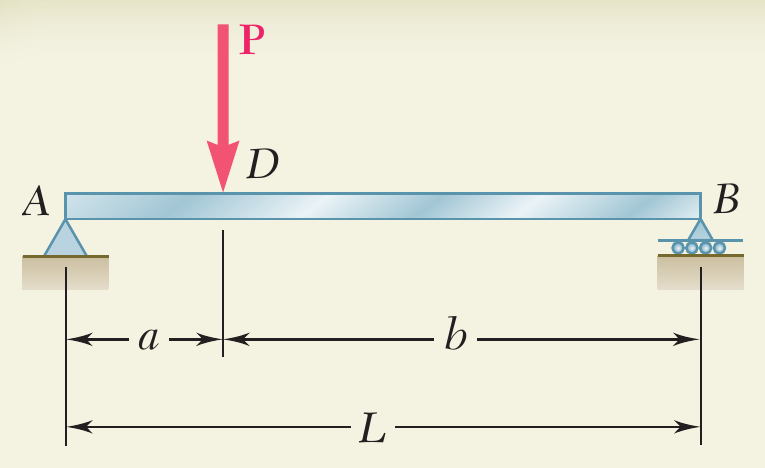
\includegraphics[width=\linewidth,height=5.5cm,keepaspectratio]{Chap_11/sp_11_2_a.png}
    \column{0.56\textwidth}
      \small
      \begin{enumerate}[a)]
        \item Chỉ kể đến ứng suất pháp do uốn, xác định năng lượng biến dạng của
              dầm với tải trọng như hình vẽ.
        \item Tính năng lượng biến dạng biết dầm là W250$\times$67,
              $P = 160\,\mathrm{kN}$, $L = 3{,}6\,\mathrm{m}$,
              $a = 0{,}9\,\mathrm{m}$, $b = 2{,}7\,\mathrm{m}$ và
              $E = 200\,\mathrm{GPa}$.
      \end{enumerate}
      \vspace{0.3em}
      \textbf{LỜI GIẢI:}
      \begin{itemize}
        \setlength{\itemsep}{0.3em}
        \item Xác định phản lực tại $A$ và $B$ từ sơ đồ vật thể tự do của toàn
              bộ dầm.
        \item Vẽ biểu đồ phân bố mô men uốn.
        \item Tích phân trên thể tích dầm để tìm năng lượng biến dạng.
        \item Áp dụng các điều kiện cụ thể đã cho để tính năng lượng biến dạng.
      \end{itemize}
  \end{columns}
\end{frame}
% ===========
\begin{frame}[t]{Bài mẫu 11.2 (tiếp)}
  \begin{columns}[T]
    \column{0.50\textwidth}
      \small
      \textbf{LỜI GIẢI:}
      \begin{itemize}
        \setlength{\itemsep}{0.6em}
        \item Xác định phản lực tại $A$ và $B$ từ sơ đồ vật thể tự do của toàn
              bộ dầm:
        \[
          R_A = \frac{Pb}{L} \qquad R_B = \frac{Pa}{L}
        \]
        \item Vẽ biểu đồ phân bố mô men uốn:
        \[
          M_1 = \frac{Pb}{L}x \qquad M_2 = \frac{Pa}{L}v
        \]
      \end{itemize}
    \column{0.48\textwidth}
      \centering
      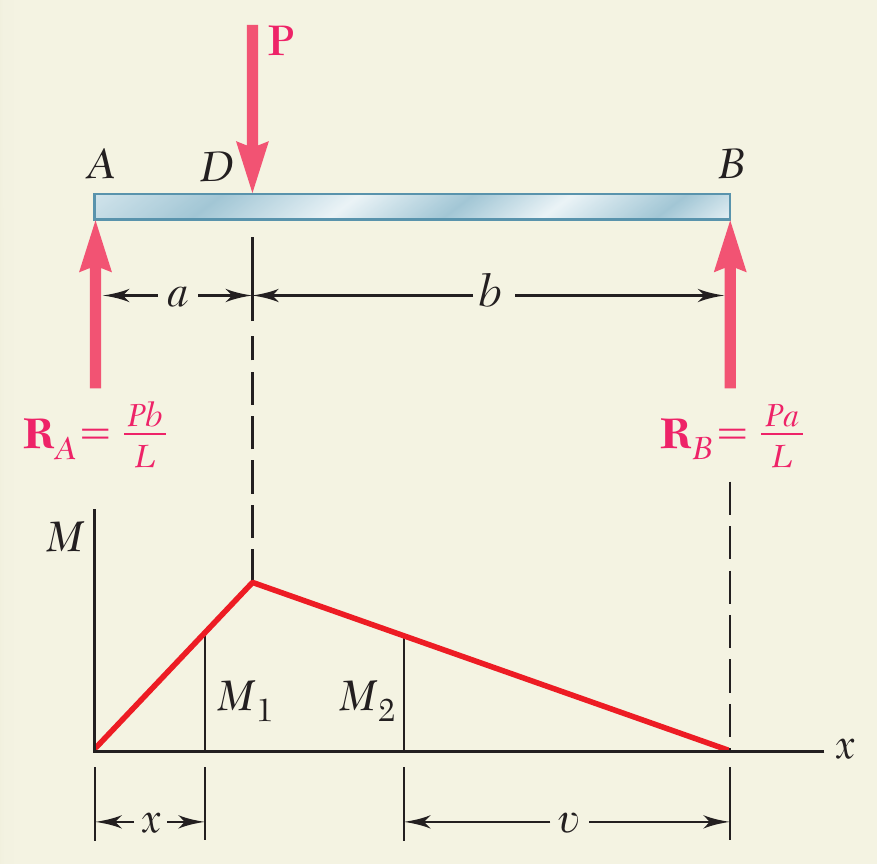
\includegraphics[width=\linewidth,height=2.9cm,keepaspectratio]{Chap_11/sp_11_2_b.png}\\[2pt]
      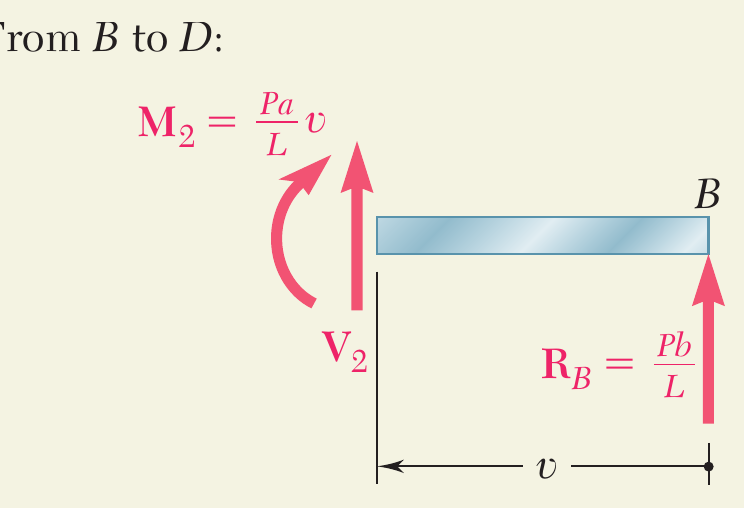
\includegraphics[width=\linewidth,height=2.9cm,keepaspectratio]{Chap_11/sp_11_2_c.png}
  \end{columns}
\end{frame}
% ===========
\begin{frame}[t]{Bài mẫu 11.2 (tiếp)}
  \begin{columns}[T]
    \column{0.62\textwidth}
      \scriptsize
      \begin{itemize}
        \setlength{\itemsep}{0.15em}
        \item Tích phân trên thể tích dầm để tìm năng lượng biến dạng.

              Trên đoạn $AD$: \ $M_1 = \dfrac{Pb}{L}x$ \qquad
              Trên đoạn $BD$: \ $M_2 = \dfrac{Pa}{L}v$
        \[
          U = \int_0^a\frac{M_1^2}{2EI}\,dx + \int_0^b\frac{M_2^2}{2EI}\,dv
        \]
        \[
          = \frac{1}{2EI}\int_0^a\left(\frac{Pb}{L}x\right)^2dx
              + \frac{1}{2EI}\int_0^b\left(\frac{Pa}{L}v\right)^2dv
        \]
        \[
          = \frac{1}{2EI}\frac{P^2}{L^2}\left(\frac{b^2a^3}{3} + \frac{a^2b^3}{3}\right)
          = \frac{P^2a^2b^2}{6EIL^2}(a + b)
        \]
        \[
          \boxed{U = \frac{P^2a^2b^2}{6EIL}}
        \]
        \item Với $P = 160\,\mathrm{kN}$, $L = 3{,}6\,\mathrm{m}$,
              $a = 0{,}9\,\mathrm{m}$, $b = 2{,}7\,\mathrm{m}$,
              $E = 200\,\mathrm{GPa}$, $I = 104\times10^{6}\,\mathrm{mm}^4$:
        \[
          U = \frac{(160\,000)^2(0{,}9)^2(2{,}7)^2}
                   {6(200\times10^{9})(104\times10^{-6})(3{,}6)}
          \qquad \boxed{U = 336\,\mathrm{N\cdot m}}
        \]
      \end{itemize}
    \column{0.36\textwidth}
      \centering
      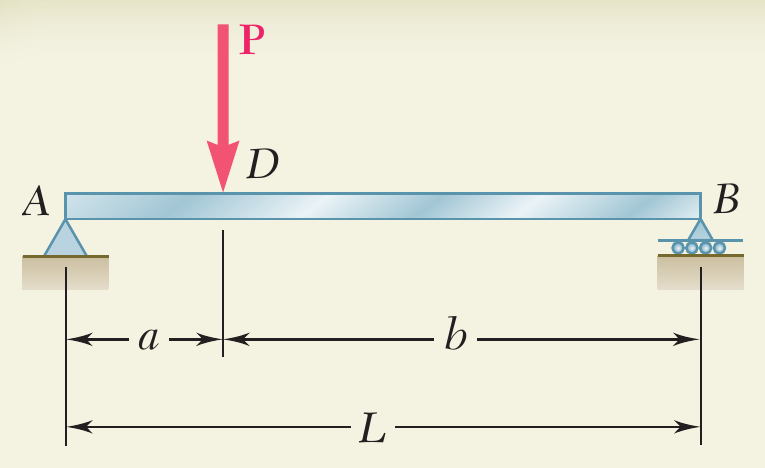
\includegraphics[width=\linewidth,height=4.7cm,keepaspectratio]{Chap_11/sp_11_2_a.png}
  \end{columns}
\end{frame}
% ===========
\section{Năng lượng biến dạng cho trạng thái ứng suất tổng quát}
\begin{frame}[t]{Năng lượng biến dạng cho trạng thái ứng suất tổng quát}
  \small
  \begin{itemize}
    \setlength{\itemsep}{0.5em}
    \item Trước đây đã tìm năng lượng biến dạng do ứng suất đơn trục và ứng suất
          tiếp phẳng. Với trạng thái ứng suất tổng quát:
    \[
      u = \tfrac{1}{2}\left(\sigma_x\varepsilon_x + \sigma_y\varepsilon_y
        + \sigma_z\varepsilon_z + \tau_{xy}\gamma_{xy} + \tau_{yz}\gamma_{yz}
        + \tau_{zx}\gamma_{zx}\right)
    \]
    \item Đối với các trục chính của vật thể đàn hồi, đẳng hướng:
    \[
      u = \frac{1}{2E}\left[\sigma_a^2 + \sigma_b^2 + \sigma_c^2
        - 2\nu(\sigma_a\sigma_b + \sigma_b\sigma_c + \sigma_c\sigma_a)\right]
        = u_v + u_d
    \]
    \[
      u_v = \frac{1 - 2\nu}{6E}(\sigma_a + \sigma_b + \sigma_c)^2
        = \text{do thay đổi thể tích}
    \]
    \[
      u_d = \frac{1}{12G}\left[(\sigma_a - \sigma_b)^2 + (\sigma_b - \sigma_c)^2
        + (\sigma_c - \sigma_a)^2\right] = \text{do thay đổi hình dáng}
    \]
    \item Cơ sở của tiêu chuẩn phá hủy năng lượng biến dạng hình dáng lớn nhất:
    \[
      u_d < (u_d)_Y = \frac{\sigma_Y^2}{6G} \quad\text{đối với mẫu thử kéo}
    \]
  \end{itemize}
\end{frame}
% ===========
\section{Tải trọng va chạm}
\begin{frame}[t]{Tải trọng va chạm}
  \begin{columns}[T]
    \column{0.70\textwidth}
      \scriptsize
      \begin{itemize}
        \setlength{\itemsep}{0.05em}
        \item Xét một thanh bị một vật có khối lượng $m$ chuyển động với vận tốc
              $v_0$ va vào đầu thanh.
        \item Thanh biến dạng do va chạm. Ứng suất đạt giá trị lớn nhất
              $\sigma_m$ rồi biến mất.
        \item Để xác định ứng suất lớn nhất $\sigma_m$:
              \begin{itemize}
                \item Giả thiết toàn bộ động năng được truyền cho kết cấu:
                      \[ U_m = \tfrac{1}{2}mv_0^2 \]
                \item Giả thiết biểu đồ ứng suất -- biến dạng nhận được từ thí
                      nghiệm tĩnh vẫn đúng khi chịu tải trọng va chạm.
              \end{itemize}
        \item Giá trị lớn nhất của năng lượng biến dạng:
        \[
          U_m = \int\frac{\sigma_m^2}{2E}\,dV
        \]
        \item Với thanh đồng chất:
        \[
          \sigma_m = \sqrt{\frac{2U_mE}{V}} = \sqrt{\frac{mv_0^2E}{V}}
        \]
      \end{itemize}
    \column{0.28\textwidth}
      \centering
      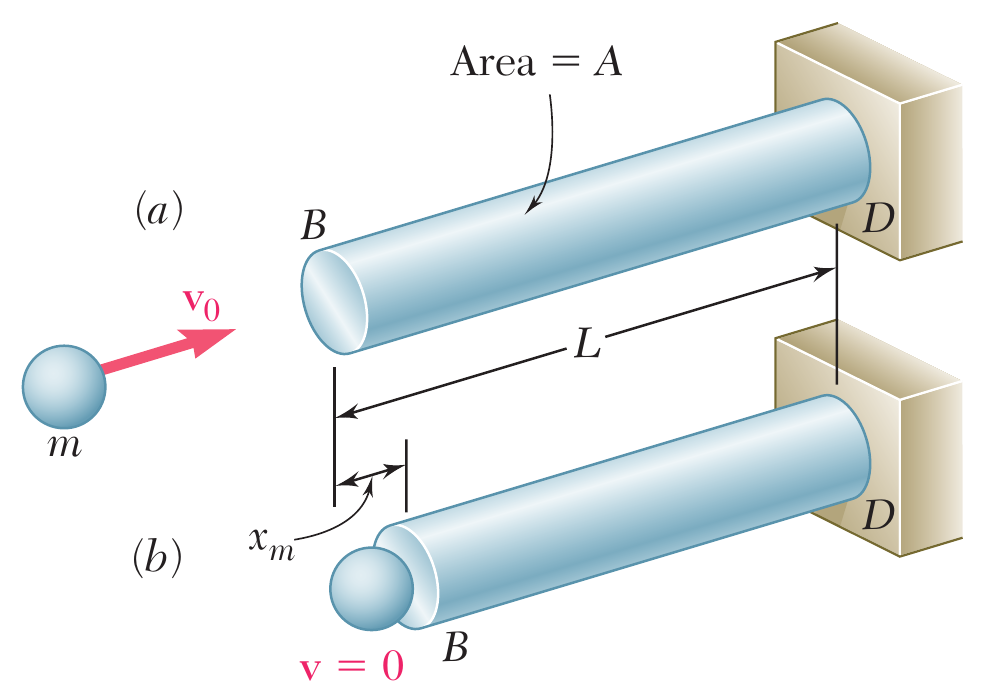
\includegraphics[width=\linewidth,height=3.4cm,keepaspectratio]{Chap_11/fig_11_22.png}
  \end{columns}
\end{frame}
% ===========
\section{Ví dụ 11.06}
\begin{frame}[t]{Ví dụ 11.06}
  \begin{columns}[T]
    \column{0.42\textwidth}
      \centering
      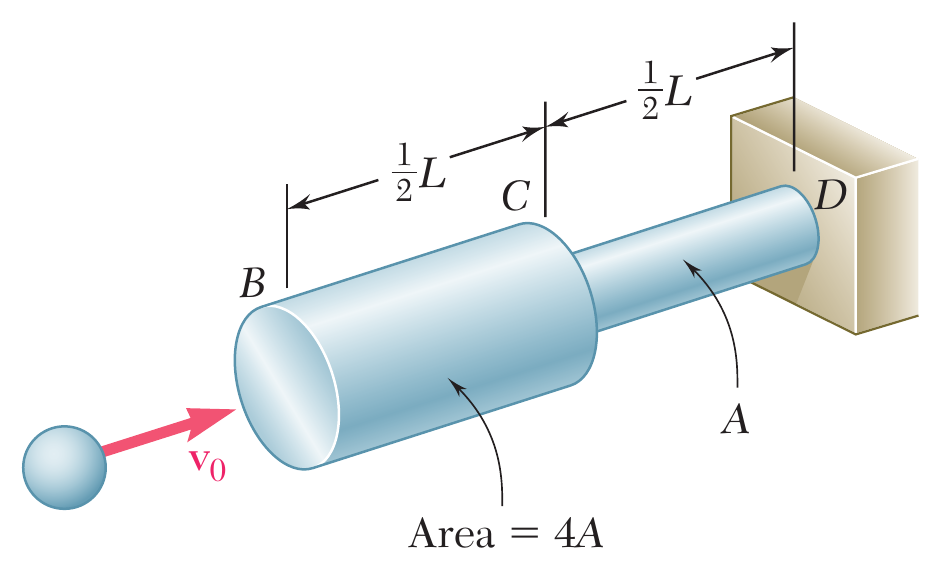
\includegraphics[width=\linewidth,height=5.5cm,keepaspectratio]{Chap_11/fig_11_23.png}
    \column{0.56\textwidth}
      \small
      Vật có khối lượng $m$ với vận tốc $v_0$ va vào đầu thanh không đồng chất
      $BCD$. Biết đường kính đoạn $BC$ gấp đôi đường kính đoạn $CD$, xác định
      giá trị lớn nhất của ứng suất pháp trong thanh.

      \vspace{0.8em}
      \textbf{LỜI GIẢI:}
      \begin{itemize}
        \setlength{\itemsep}{0.4em}
        \item Do đường kính thay đổi, phân bố ứng suất pháp không đều.
        \item Tìm tải trọng tĩnh $P_m$ gây ra cùng năng lượng biến dạng như va
              chạm.
        \item Tính ứng suất lớn nhất do tải trọng tĩnh $P_m$ gây ra.
      \end{itemize}
  \end{columns}
\end{frame}
% ===========
\begin{frame}[t]{Ví dụ 11.06 (tiếp)}
  \begin{columns}[T]
    \column{0.58\textwidth}
      \footnotesize
      \textbf{LỜI GIẢI:}
      \begin{itemize}
        \setlength{\itemsep}{0.20em}
        \item Do đường kính thay đổi, phân bố ứng suất pháp không đều:
        \[
          U_m = \tfrac{1}{2}mv_0^2
          \qquad
          U_m = \int\frac{\sigma^2}{2E}\,dV \neq \frac{\sigma_m^2V}{2E}
        \]
        \item Tìm tải trọng tĩnh $P_m$ gây ra cùng năng lượng biến dạng như va
              chạm:
        \[
          U_m = \frac{P_m^2(L/2)}{2AE} + \frac{P_m^2(L/2)}{2(4A)E}
            = \frac{5}{16}\frac{P_m^2L}{AE}
        \]
        \[
          P_m = \sqrt{\frac{16}{5}\frac{U_mAE}{L}}
        \]
        \item Tính ứng suất lớn nhất do tải trọng tĩnh $P_m$:
        \[
          \sigma_m = \frac{P_m}{A} = \sqrt{\frac{16}{5}\frac{U_mE}{AL}}
          \qquad
          \boxed{\sigma_m = \sqrt{\frac{8}{5}\frac{mv_0^2E}{AL}}}
        \]
      \end{itemize}
    \column{0.40\textwidth}
      \centering
      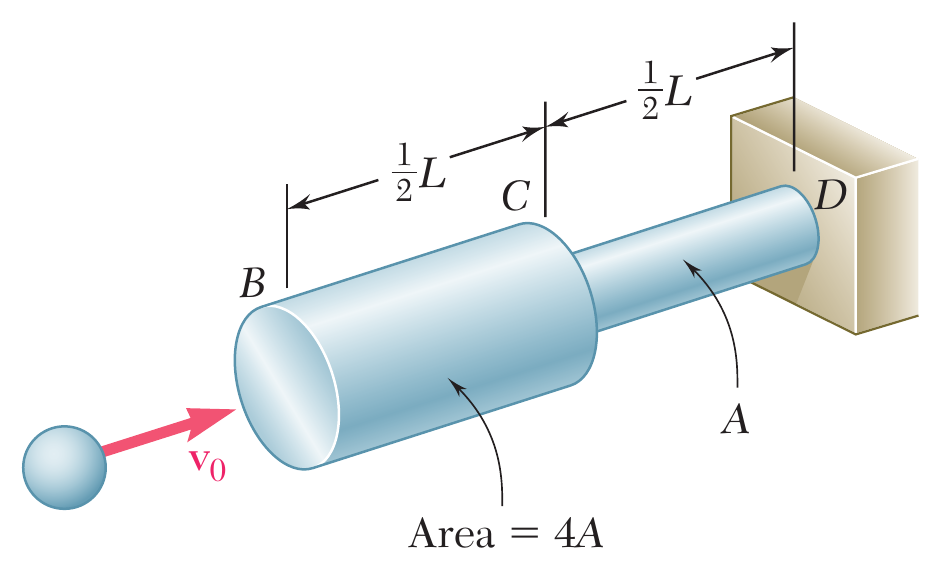
\includegraphics[width=\linewidth,height=4.7cm,keepaspectratio]{Chap_11/fig_11_23.png}
  \end{columns}
\end{frame}
% ===========
\section{Ví dụ 11.07}
\begin{frame}[t]{Ví dụ 11.07}
  \begin{columns}[T]
    \column{0.42\textwidth}
      \centering
      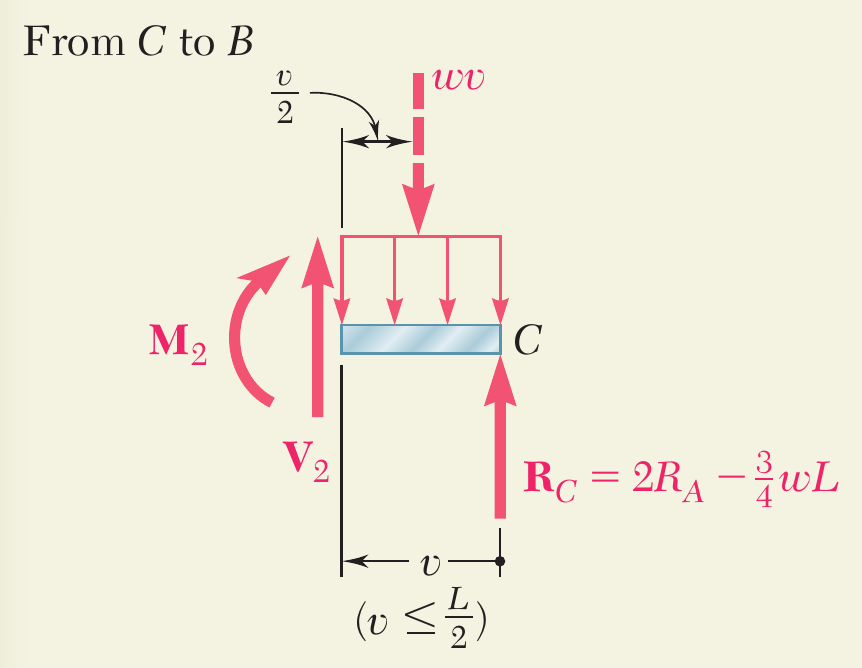
\includegraphics[width=\linewidth,height=5.5cm,keepaspectratio]{Chap_11/sp_11_7.png}
    \column{0.56\textwidth}
      \small
      Một khối có trọng lượng $W$ được thả rơi từ độ cao $h$ xuống đầu tự do
      của dầm công xôn. Xác định giá trị lớn nhất của ứng suất trong dầm.

      \vspace{0.8em}
      \textbf{LỜI GIẢI:}
      \begin{itemize}
        \setlength{\itemsep}{0.4em}
        \item Ứng suất pháp thay đổi tuyến tính dọc theo chiều dài dầm và trên
              mặt cắt ngang.
        \item Tìm tải trọng tĩnh $P_m$ gây ra cùng năng lượng biến dạng như va
              chạm.
        \item Tính ứng suất lớn nhất do tải trọng tĩnh $P_m$ gây ra.
      \end{itemize}
  \end{columns}
\end{frame}
% ===========
\begin{frame}[t]{Ví dụ 11.07 (tiếp)}
  \begin{columns}[T]
    \column{0.58\textwidth}
      \small
      \textbf{LỜI GIẢI:}
      \begin{itemize}
        \setlength{\itemsep}{0.4em}
        \item Ứng suất pháp thay đổi tuyến tính dọc theo chiều dài dầm và trên
              mặt cắt ngang:
        \[
          U_m = Wh \qquad
          U_m = \int\frac{\sigma^2}{2E}\,dV \neq \frac{\sigma_m^2V}{2E}
        \]
        \item Tìm tải trọng tĩnh $P_m$ gây ra cùng năng lượng biến dạng như va
              chạm. Với dầm công xôn chịu lực ở đầu tự do:
        \[
          U_m = \frac{P_m^2L^3}{6EI}
          \qquad
          P_m = \sqrt{\frac{6U_mEI}{L^3}}
        \]
        \item Tính ứng suất lớn nhất do tải trọng tĩnh $P_m$:
        \[
          \sigma_m = \frac{|M_m|c}{I} = \frac{P_mLc}{I}
            = \sqrt{\frac{6U_mE}{L(I/c^2)}}
            = \sqrt{\frac{6WhE}{L(I/c^2)}}
        \]
      \end{itemize}
    \column{0.40\textwidth}
      \centering
      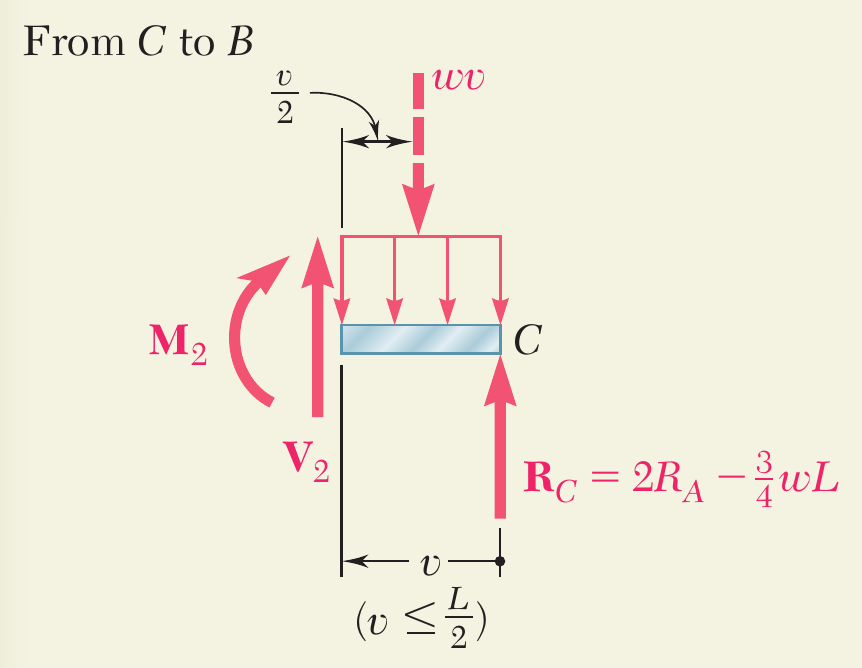
\includegraphics[width=\linewidth,height=5.5cm,keepaspectratio]{Chap_11/sp_11_7.png}
  \end{columns}
\end{frame}
% ===========
\section{Thiết kế chịu tải trọng va chạm}
\begin{frame}[t]{Thiết kế chịu tải trọng va chạm}
  \begin{columns}[T]
    \column{0.62\textwidth}
      \footnotesize
      \begin{itemize}
        \setlength{\itemsep}{0.3em}
        \item Với thanh đồng chất:
        \[
          \sigma_m = \sqrt{\frac{2U_mE}{V}}
        \]
        \item Với thanh không đồng chất:
        \[
          V = 4A(L/2) + A(L/2) = 5AL/2
        \]
        \[
          \sigma_m = \sqrt{\frac{16U_mE}{5AL}} = \sqrt{\frac{8U_mE}{V}}
        \]
        \item Với dầm công xôn:
        \[
          L(I/c^2) = L\left(\tfrac{1}{4}\pi c^4/c^2\right) = \tfrac{1}{4}(\pi c^2L)
            = \tfrac{1}{4}V
        \]
        \[
          \sigma_m = \sqrt{\frac{6U_mE}{L(I/c^2)}} = \sqrt{\frac{24U_mE}{V}}
        \]
      \end{itemize}
    \column{0.36\textwidth}
      \centering
      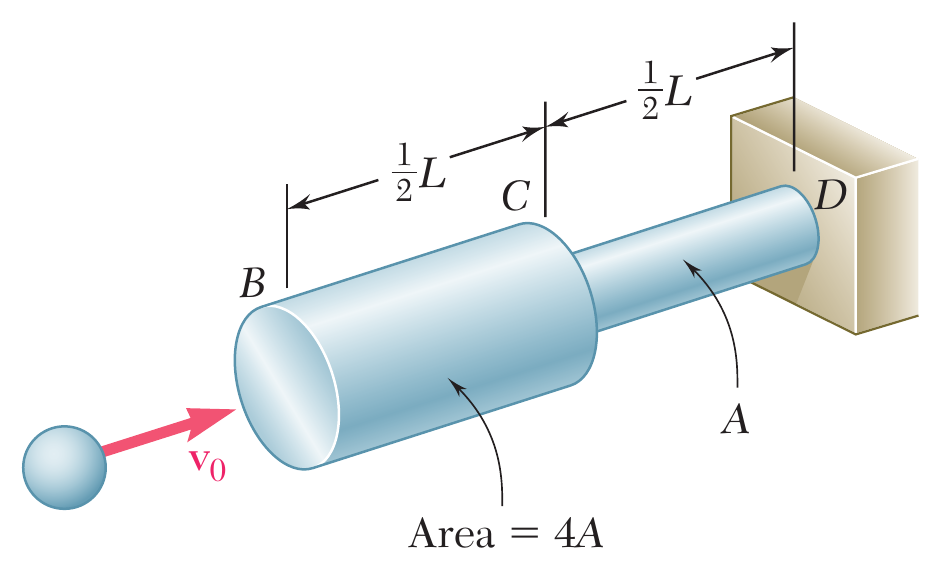
\includegraphics[width=\linewidth,height=2.2cm,keepaspectratio]{Chap_11/fig_11_23.png}\\[2pt]
      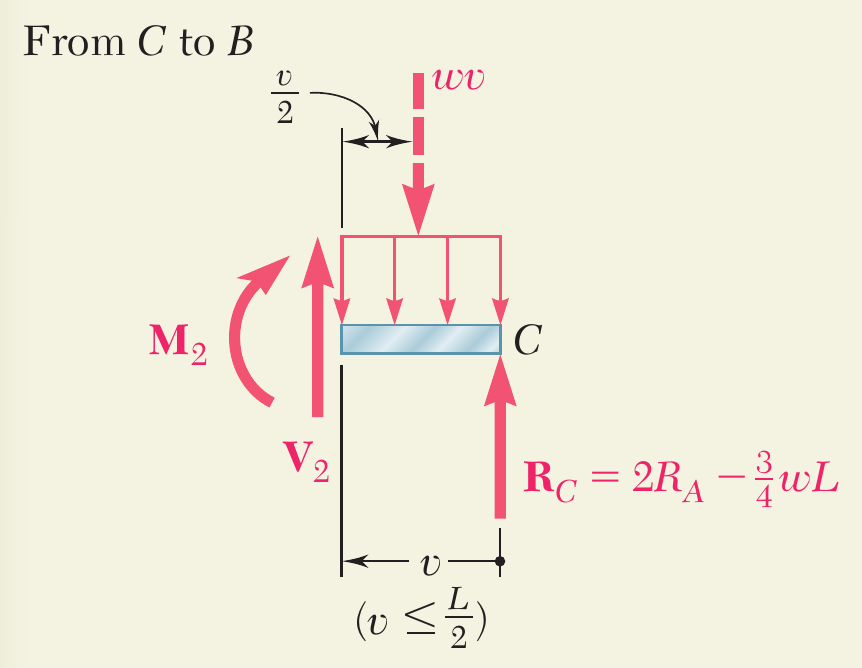
\includegraphics[width=\linewidth,height=2.2cm,keepaspectratio]{Chap_11/sp_11_7.png}
      \raggedright\footnotesize
      Ứng suất lớn nhất được giảm nhờ:
      \begin{itemize}
        \item ứng suất phân bố đều
        \item mô đun đàn hồi thấp kết hợp với giới hạn chảy cao
        \item thể tích lớn
      \end{itemize}
  \end{columns}
\end{frame}
% ===========
\section{Công và năng lượng dưới tác dụng của một tải trọng}
\begin{frame}[t]{Công và năng lượng dưới tác dụng của một tải trọng}
  \begin{columns}[T]
    \column{0.60\textwidth}
      \footnotesize
      \begin{itemize}
        \setlength{\itemsep}{0.3em}
        \item Trước đây, ta tìm năng lượng biến dạng bằng cách tích phân mật độ
              năng lượng trên thể tích. Với thanh đồng chất:
        \[
          U = \int u\,dV = \int\frac{\sigma^2}{2E}\,dV
            = \int_0^L\frac{(P_1/A)^2}{2E}A\,dx = \frac{P_1^2L}{2AE}
        \]
        \item Năng lượng biến dạng cũng có thể được tìm từ công của tải trọng
              đơn $P_1$:
        \[
          U = \int_0^{x_1}P\,dx
        \]
        \item Với biến dạng đàn hồi:
        \[
          U = \int_0^{x_1}P\,dx = \int_0^{x_1}kx\,dx = \tfrac{1}{2}kx_1^2
            = \tfrac{1}{2}P_1x_1
        \]
        \item Biết quan hệ giữa lực và chuyển vị:
        \[
          x_1 = \frac{P_1L}{AE}
          \qquad
          U = \tfrac{1}{2}P_1\left(\frac{P_1L}{AE}\right) = \frac{P_1^2L}{2AE}
        \]
      \end{itemize}
    \column{0.38\textwidth}
      \centering
      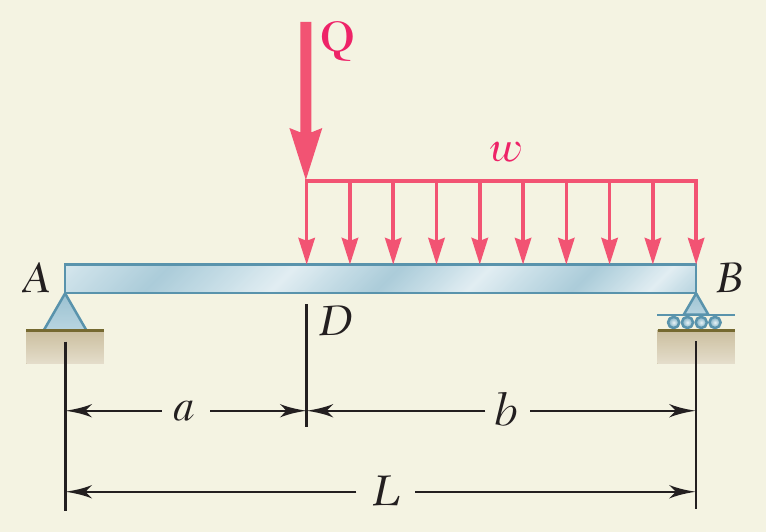
\includegraphics[width=\linewidth,height=5.5cm,keepaspectratio]{Chap_11/sp_11_6_a.png}
  \end{columns}
\end{frame}
% ===========
\begin{frame}[t]{Công và năng lượng dưới tác dụng của một tải trọng (tiếp)}
  \begin{columns}[T]
    \column{0.60\textwidth}
      \small
      Năng lượng biến dạng có thể được tìm từ công của các loại tải trọng tập
      trung đơn khác.
      \begin{itemize}
        \setlength{\itemsep}{0.5em}
        \item Lực ngang:
        \[
          U = \int_0^{y_1}P\,dy = \tfrac{1}{2}P_1y_1
            = \tfrac{1}{2}P_1\left(\frac{P_1L^3}{3EI}\right) = \frac{P_1^2L^3}{6EI}
        \]
        \item Ngẫu lực uốn:
        \[
          U = \int_0^{\theta_1}M\,d\theta = \tfrac{1}{2}M_1\theta_1
            = \tfrac{1}{2}M_1\left(\frac{M_1L}{EI}\right) = \frac{M_1^2L}{2EI}
        \]
        \item Ngẫu lực xoắn:
        \[
          U = \int_0^{\phi_1}T\,d\phi = \tfrac{1}{2}T_1\phi_1
            = \tfrac{1}{2}T_1\left(\frac{T_1L}{JG}\right) = \frac{T_1^2L}{2JG}
        \]
      \end{itemize}
    \column{0.38\textwidth}
      \centering
      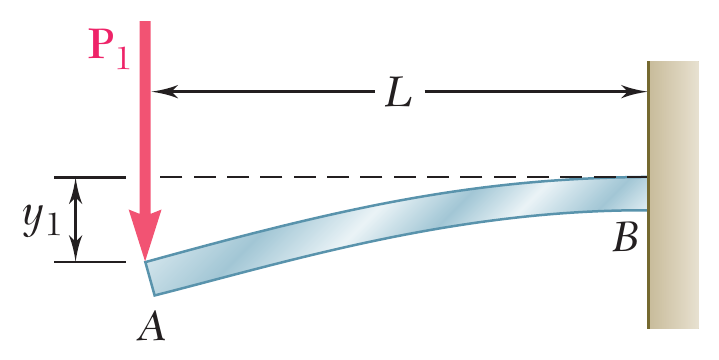
\includegraphics[width=\linewidth,height=1.9cm,keepaspectratio]{Chap_11/fig_11_25.png}\\[2pt]
      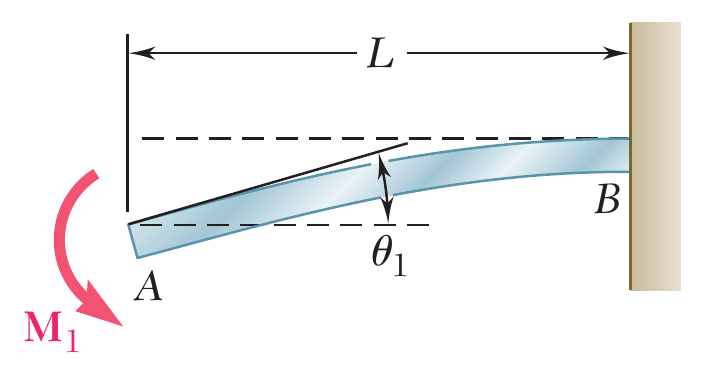
\includegraphics[width=\linewidth,height=1.9cm,keepaspectratio]{Chap_11/fig_11_26.png}\\[2pt]
      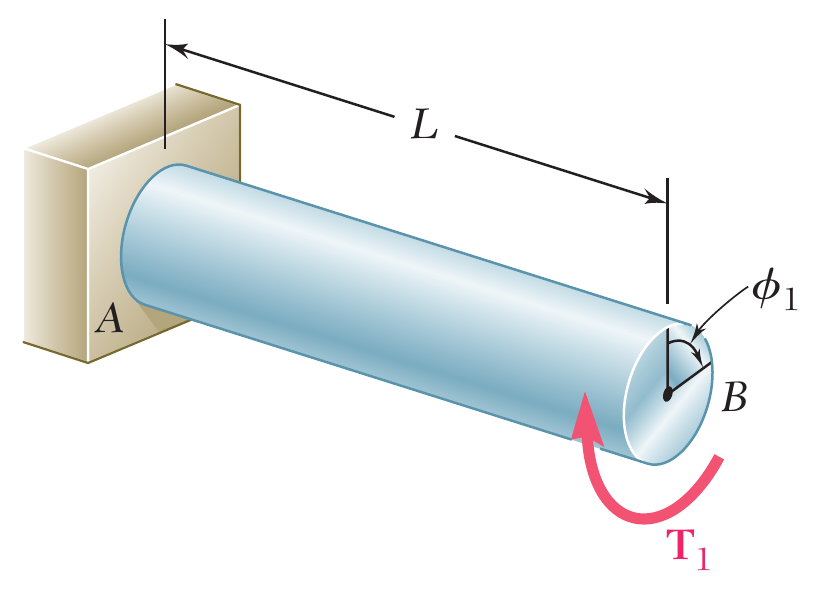
\includegraphics[width=\linewidth,height=1.9cm,keepaspectratio]{Chap_11/fig_11_27.png}
  \end{columns}
\end{frame}
% ===========
\section{Chuyển vị dưới tác dụng của một tải trọng}
\begin{frame}[t]{Chuyển vị dưới tác dụng của một tải trọng}
  \begin{columns}[T]
    \column{0.60\textwidth}
      \footnotesize
      \begin{itemize}
        \setlength{\itemsep}{0.20em}
        \item Nếu biết năng lượng biến dạng của kết cấu do một tải trọng tập
              trung đơn, có thể dùng đẳng thức giữa công của tải trọng và năng
              lượng để tìm chuyển vị.
        \item Từ hình học đã cho: \quad $L_{BC} = 0{,}6l$, \quad $L_{BD} = 0{,}8l$
        \item Từ tĩnh học: \quad $F_{BC} = +0{,}6P$, \quad $F_{BD} = -0{,}8P$
        \item Năng lượng biến dạng của kết cấu:
        \[
          U = \frac{F_{BC}^2L_{BC}}{2AE} + \frac{F_{BD}^2L_{BD}}{2AE}
            = \frac{P^2l\left[(0{,}6)^3 + (0{,}8)^3\right]}{2AE}
        \]
        \[
          U = 0{,}364\frac{P^2l}{AE}
        \]
        \item Cân bằng công và năng lượng biến dạng:
        \[
          U = 0{,}364\frac{P^2l}{AE} = \tfrac{1}{2}Py_B
          \qquad
          \boxed{y_B = 0{,}728\frac{Pl}{AE}}
        \]
      \end{itemize}
    \column{0.38\textwidth}
      \centering
      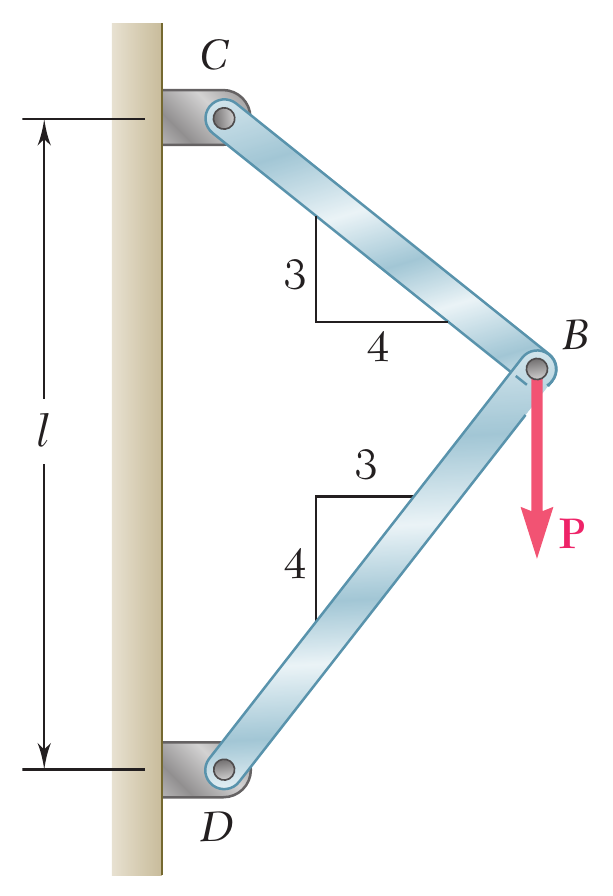
\includegraphics[width=\linewidth,height=4.7cm,keepaspectratio]{Chap_11/fig_11_44.png}
  \end{columns}
\end{frame}
% ===========
\section{Bài mẫu 11.4}
\begin{frame}[t]{Bài mẫu 11.4}
  \begin{columns}[T]
    \column{0.42\textwidth}
      \centering
      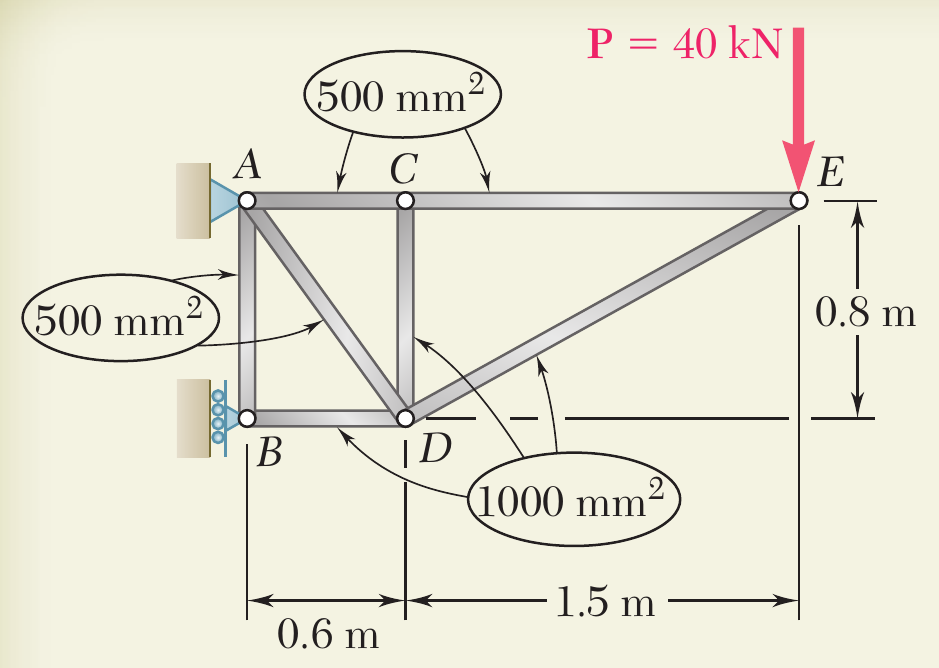
\includegraphics[width=\linewidth,height=5.5cm,keepaspectratio]{Chap_11/sp_11_4_a.png}
    \column{0.56\textwidth}
      \small
      Các thanh của giàn như hình vẽ là các đoạn ống nhôm với diện tích mặt cắt
      ngang như ghi trên hình. Với $E = 73\,\mathrm{GPa}$, xác định chuyển vị
      thẳng đứng của điểm $E$ do tải trọng $P$ gây ra.

      \vspace{0.5em}
      \textbf{LỜI GIẢI:}
      \begin{itemize}
        \setlength{\itemsep}{0.3em}
        \item Tìm phản lực tại $A$ và $B$ từ sơ đồ vật thể tự do của toàn bộ
              giàn.
        \item Áp dụng phương pháp tách nút để xác định lực dọc trong mỗi thanh.
        \item Tính năng lượng biến dạng của giàn do tải trọng $P$.
        \item Cân bằng năng lượng biến dạng với công của $P$ và giải ra chuyển
              vị.
      \end{itemize}
  \end{columns}
\end{frame}
% ===========
\begin{frame}[t]{Bài mẫu 11.4 (tiếp)}
  \begin{columns}[T]
    \column{0.50\textwidth}
      \small
      \textbf{LỜI GIẢI:}
      \begin{itemize}
        \setlength{\itemsep}{0.5em}
        \item Tìm phản lực tại $A$ và $B$ từ sơ đồ vật thể tự do của toàn bộ
              giàn:
        \[
          A_x = -\frac{21P}{8} \qquad A_y = P \qquad B = \frac{21P}{8}
        \]
        \item Áp dụng phương pháp tách nút để xác định lực dọc trong mỗi thanh:
        \[
          \begin{aligned}
            F_{AB} &= 0 & F_{AC} &= +\tfrac{15}{8}P\\
            F_{AD} &= +\tfrac{5}{4}P & F_{BD} &= -\tfrac{21}{8}P\\
            F_{CD} &= 0 & F_{CE} &= +\tfrac{15}{8}P\\
            F_{DE} &= -\tfrac{17}{8}P & &
          \end{aligned}
        \]
      \end{itemize}
    \column{0.48\textwidth}
      \centering
      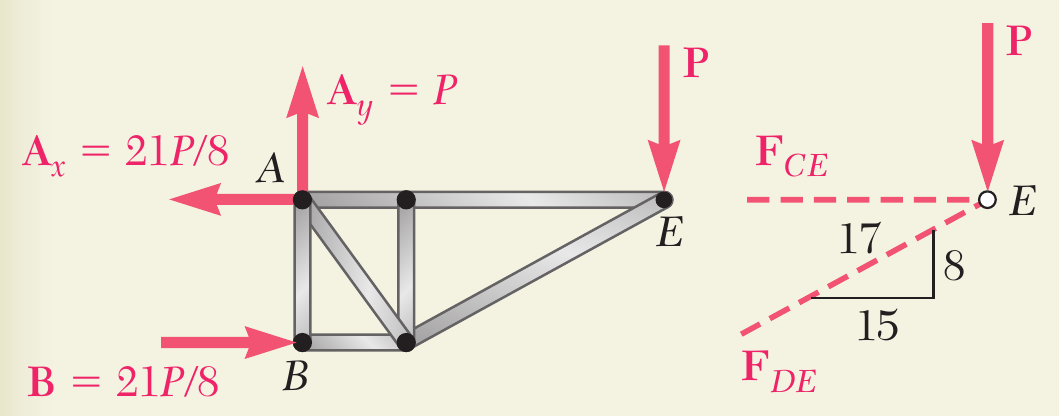
\includegraphics[width=\linewidth,height=2.9cm,keepaspectratio]{Chap_11/sp_11_4_b.png}\\[2pt]
      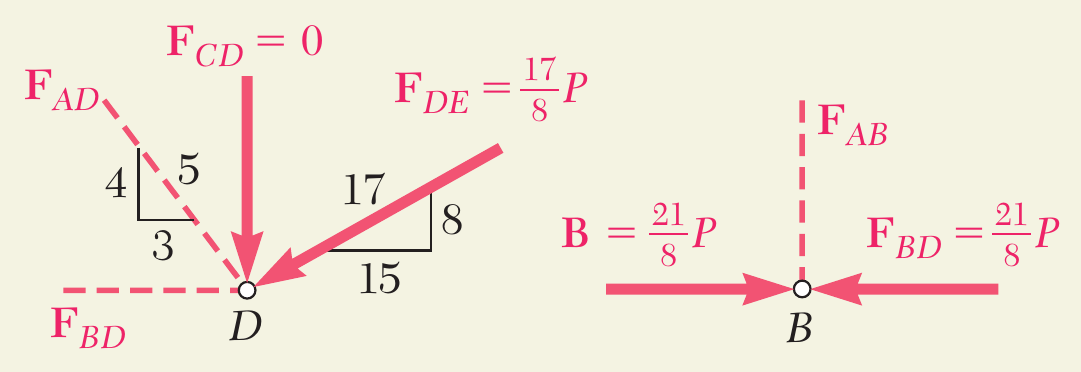
\includegraphics[width=\linewidth,height=2.9cm,keepaspectratio]{Chap_11/sp_11_4_c.png}
  \end{columns}
\end{frame}
% ===========
\begin{frame}[t]{Bài mẫu 11.4 (tiếp)}
  \begin{columns}[T]
    \column{0.58\textwidth}
      \small
      \begin{itemize}
        \setlength{\itemsep}{0.5em}
        \item Tính năng lượng biến dạng của giàn do tải trọng $P$:
        \[
          U = \sum\frac{F_i^2L_i}{2A_iE} = \frac{1}{2E}\sum\frac{F_i^2L_i}{A_i}
            = \frac{1}{2E}\left(29\,700P^2\right)
        \]
        \item Cân bằng năng lượng biến dạng với công của $P$ và giải ra chuyển
              vị:
        \[
          \tfrac{1}{2}Py_E = U
          \qquad
          y_E = \frac{2U}{P} = \frac{2}{P}\left(\frac{29\,700P^2}{2E}\right)
        \]
        \[
          y_E = \frac{(29{,}7\times10^{3})(40\times10^{3})}{73\times10^{9}}
          \qquad \boxed{y_E = 16{,}27\,\mathrm{mm}\downarrow}
        \]
      \end{itemize}
    \column{0.40\textwidth}
      \centering
      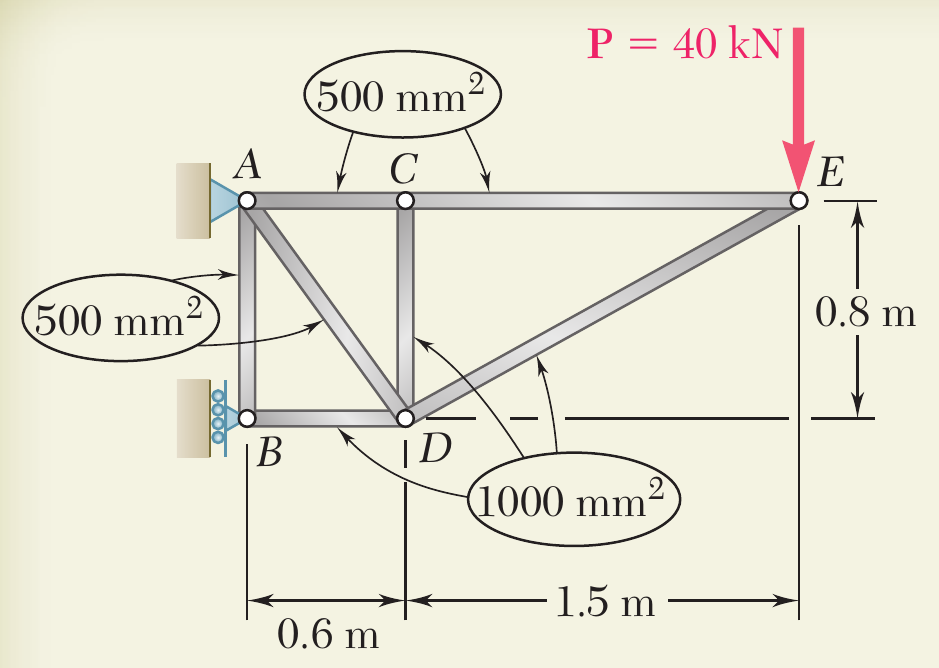
\includegraphics[width=\linewidth,height=5.5cm,keepaspectratio]{Chap_11/sp_11_4_a.png}
  \end{columns}
\end{frame}
% ===========
\section{Công và năng lượng dưới tác dụng của nhiều tải trọng}
\begin{frame}[t]{Công và năng lượng dưới tác dụng của nhiều tải trọng}
  \begin{columns}[T]
    \column{0.60\textwidth}
      \small
      \begin{itemize}
        \setlength{\itemsep}{0.4em}
        \item Chuyển vị của dầm đàn hồi chịu hai tải trọng tập trung:
        \[
          x_1 = x_{11} + x_{12} = \alpha_{11}P_1 + \alpha_{12}P_2
        \]
        \[
          x_2 = x_{21} + x_{22} = \alpha_{21}P_1 + \alpha_{22}P_2
        \]
        \item Tính năng lượng biến dạng của dầm bằng công thực hiện khi đặt
              chậm $P_1$ rồi đến $P_2$:
        \[
          U = \tfrac{1}{2}\left(\alpha_{11}P_1^2 + 2\alpha_{12}P_1P_2 + \alpha_{22}P_2^2\right)
        \]
        \item Đảo ngược thứ tự đặt tải:
        \[
          U = \tfrac{1}{2}\left(\alpha_{22}P_2^2 + 2\alpha_{21}P_2P_1 + \alpha_{11}P_1^2\right)
        \]
        \item Hai biểu thức năng lượng biến dạng phải tương đương. Suy ra
              $\alpha_{12} = \alpha_{21}$ (\emph{định lý tương hỗ Maxwell}).
      \end{itemize}
    \column{0.38\textwidth}
      \centering
      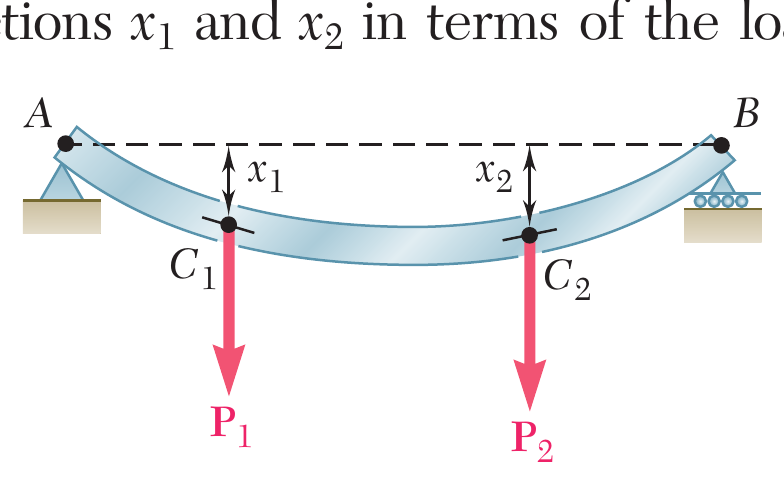
\includegraphics[width=\linewidth,height=2.9cm,keepaspectratio]{Chap_11/fig_11_33.png}\\[2pt]
      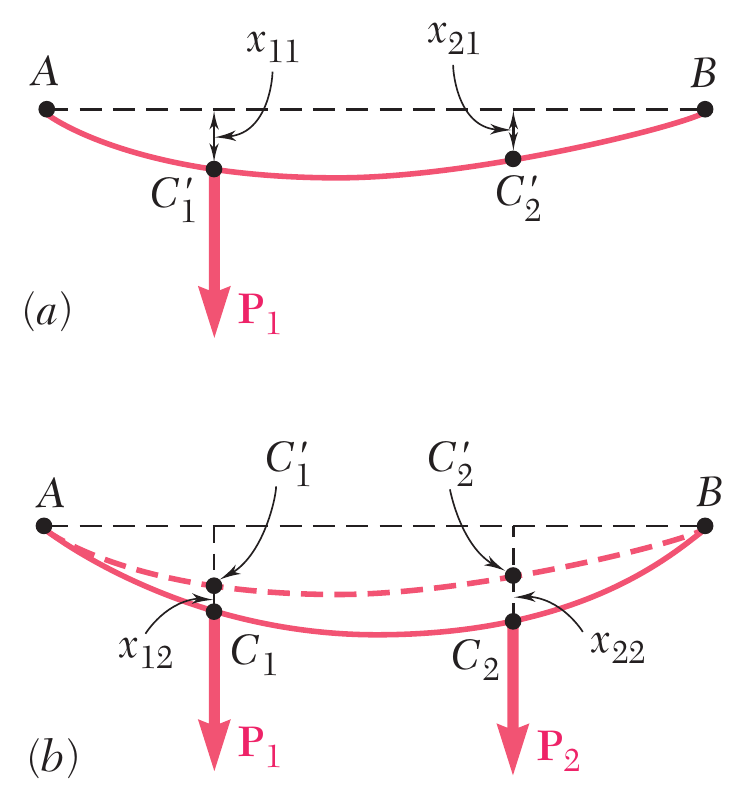
\includegraphics[width=\linewidth,height=2.9cm,keepaspectratio]{Chap_11/fig_11_36.png}
  \end{columns}
\end{frame}
% ===========
\section{Định lý Castigliano}
\begin{frame}[t]{Định lý Castigliano}
  \begin{columns}[T]
    \column{0.58\textwidth}
      \small
      \begin{itemize}
        \setlength{\itemsep}{0.5em}
        \item Năng lượng biến dạng của một kết cấu đàn hồi bất kỳ chịu hai tải
              trọng tập trung:
        \[
          U = \tfrac{1}{2}\left(\alpha_{11}P_1^2 + 2\alpha_{12}P_1P_2 + \alpha_{22}P_2^2\right)
        \]
        \item Đạo hàm theo các tải trọng:
        \[
          \frac{\partial U}{\partial P_1} = \alpha_{11}P_1 + \alpha_{12}P_2 = x_1
        \]
        \[
          \frac{\partial U}{\partial P_2} = \alpha_{12}P_1 + \alpha_{22}P_2 = x_2
        \]
        \item \textbf{Định lý Castigliano:} Với kết cấu đàn hồi chịu $n$ tải
              trọng, chuyển vị $x_j$ của điểm đặt $P_j$ có thể được biểu diễn
              là:
        \[
          x_j = \frac{\partial U}{\partial P_j}
          \qquad
          \theta_j = \frac{\partial U}{\partial M_j}
          \qquad
          \phi_j = \frac{\partial U}{\partial T_j}
        \]
      \end{itemize}
    \column{0.40\textwidth}
      \centering
      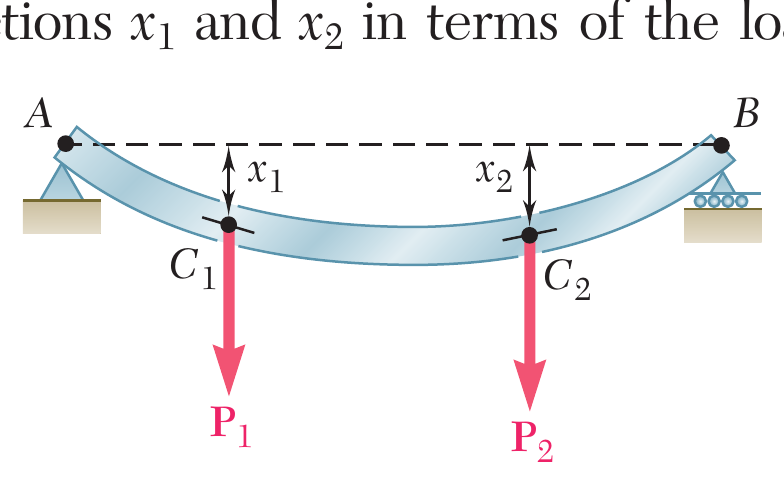
\includegraphics[width=\linewidth,height=5.5cm,keepaspectratio]{Chap_11/fig_11_33.png}
  \end{columns}
\end{frame}
% ===========
\section{Tính chuyển vị bằng định lý Castigliano}
\begin{frame}[t]{Tính chuyển vị bằng định lý Castigliano}
  \begin{columns}[T]
    \column{0.58\textwidth}
      \small
      \begin{itemize}
        \setlength{\itemsep}{0.5em}
        \item Việc áp dụng định lý Castigliano được đơn giản hóa nếu thực hiện
              phép đạo hàm theo tải trọng $P_j$ trước khi tích phân hoặc lấy
              tổng để tìm năng lượng biến dạng $U$.
        \item Trường hợp dầm:
        \[
          U = \int_0^L\frac{M^2}{2EI}\,dx
          \qquad
          x_j = \frac{\partial U}{\partial P_j}
            = \int_0^L\frac{M}{EI}\frac{\partial M}{\partial P_j}\,dx
        \]
        \item Trường hợp giàn:
        \[
          U = \sum_{i=1}^{n}\frac{F_i^2L_i}{2A_iE}
          \qquad
          x_j = \frac{\partial U}{\partial P_j}
            = \sum_{i=1}^{n}\frac{F_iL_i}{A_iE}\frac{\partial F_i}{\partial P_j}
        \]
      \end{itemize}
    \column{0.40\textwidth}
      \centering
      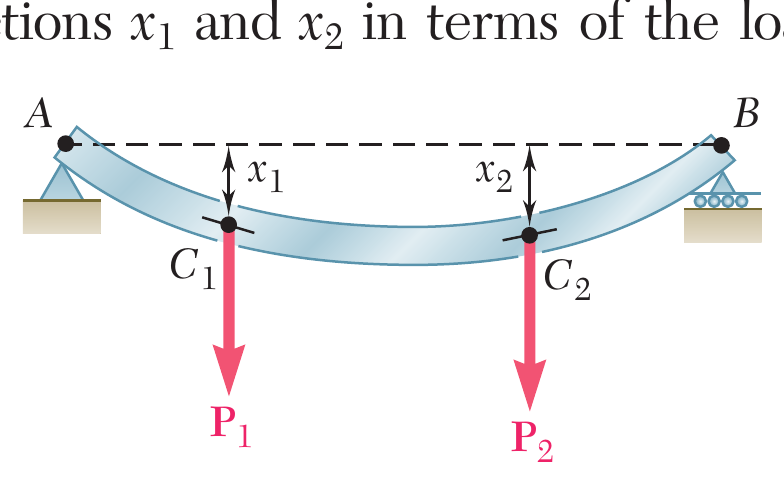
\includegraphics[width=\linewidth,height=2.9cm,keepaspectratio]{Chap_11/fig_11_33.png}\\[2pt]
      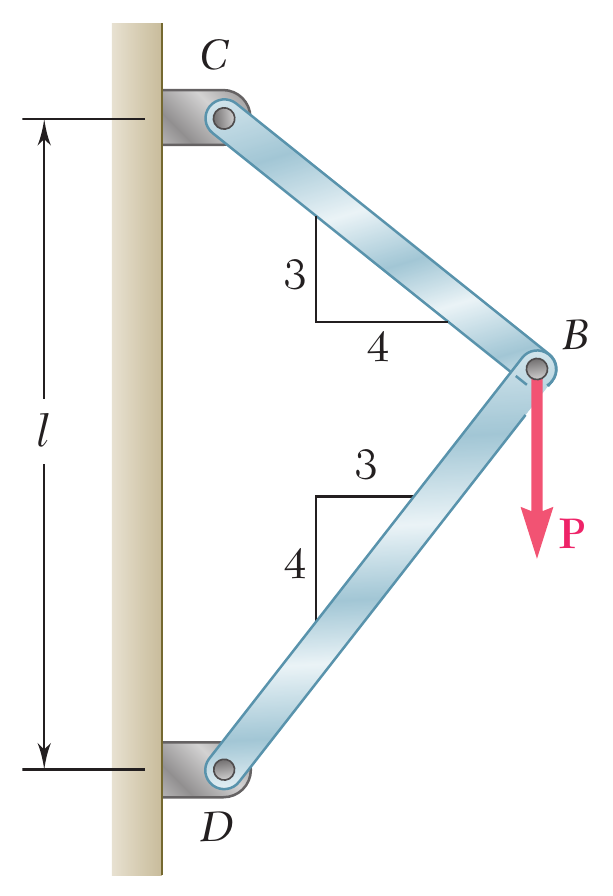
\includegraphics[width=\linewidth,height=2.9cm,keepaspectratio]{Chap_11/fig_11_44.png}
  \end{columns}
\end{frame}
% ===========
\section{Bài mẫu 11.5}
\begin{frame}[t]{Bài mẫu 11.5}
  \begin{columns}[T]
    \column{0.42\textwidth}
      \centering
      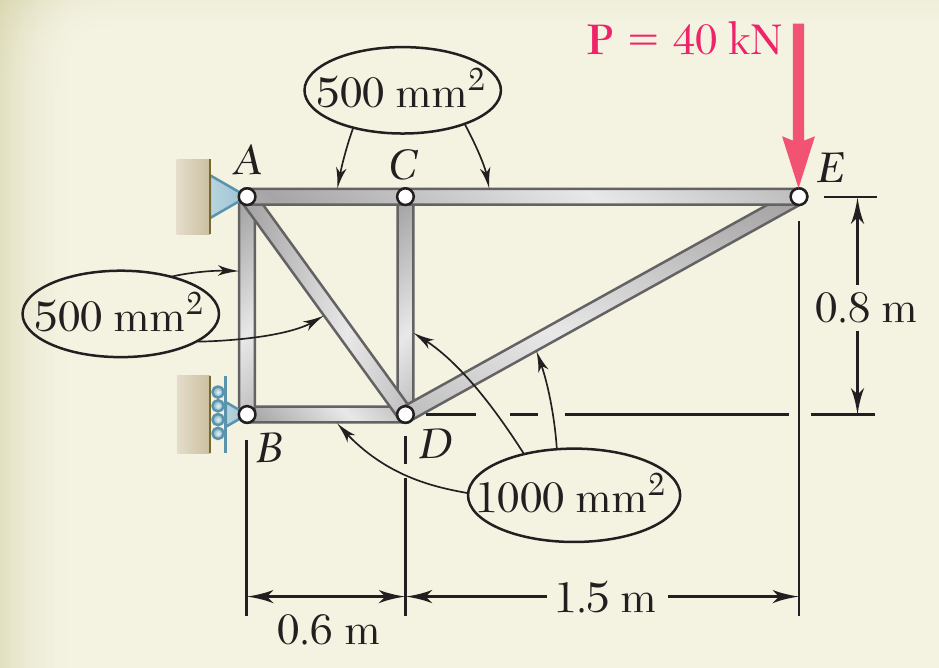
\includegraphics[width=\linewidth,height=5.5cm,keepaspectratio]{Chap_11/sp_11_5_a.png}
    \column{0.56\textwidth}
      \footnotesize
      Các thanh của giàn như hình vẽ là các đoạn ống nhôm với diện tích mặt cắt
      ngang như ghi trên hình. Với $E = 73\,\mathrm{GPa}$, xác định chuyển vị
      thẳng đứng của nút $C$ do tải trọng $P$ gây ra.

      \vspace{0.5em}
      \textbf{LỜI GIẢI:}
      \begin{itemize}
        \setlength{\itemsep}{0.3em}
        \item Để áp dụng định lý Castigliano, đặt một tải trọng giả thẳng đứng
              $Q$ tại $C$. Tìm phản lực tại $A$ và $B$ do tải trọng giả từ sơ đồ
              vật thể tự do của toàn bộ giàn.
        \item Áp dụng phương pháp tách nút để xác định lực dọc trong mỗi thanh
              do $Q$.
        \item Kết hợp với kết quả Bài mẫu 11.4 để tính đạo hàm theo $Q$ của năng
              lượng biến dạng của giàn do các tải trọng $P$ và $Q$.
        \item Cho $Q = 0$, tính giá trị đạo hàm, chính là chuyển vị cần tìm
              tại $C$.
      \end{itemize}
  \end{columns}
\end{frame}
% ===========
\begin{frame}[t]{Bài mẫu 11.5 (tiếp)}
  \begin{columns}[T]
    \column{0.50\textwidth}
      \small
      \textbf{LỜI GIẢI:}
      \begin{itemize}
        \setlength{\itemsep}{0.5em}
        \item Tìm phản lực tại $A$ và $B$ do tải trọng giả $Q$ tại $C$ từ sơ đồ
              vật thể tự do của toàn bộ giàn:
        \[
          A_x = -\tfrac{3}{4}Q \qquad A_y = Q \qquad B = \tfrac{3}{4}Q
        \]
        \item Áp dụng phương pháp tách nút để xác định lực dọc trong mỗi thanh
              do $Q$:
        \[
          \begin{aligned}
            F_{CE} &= F_{DE} = 0\\
            F_{AC} &= 0; \quad F_{CD} = -Q\\
            F_{AB} &= 0; \quad F_{BD} = -\tfrac{3}{4}Q
          \end{aligned}
        \]
      \end{itemize}
    \column{0.48\textwidth}
      \centering
      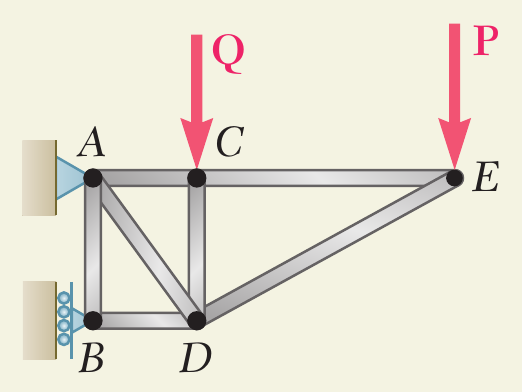
\includegraphics[width=\linewidth,height=1.9cm,keepaspectratio]{Chap_11/sp_11_5_b.png}\\[2pt]
      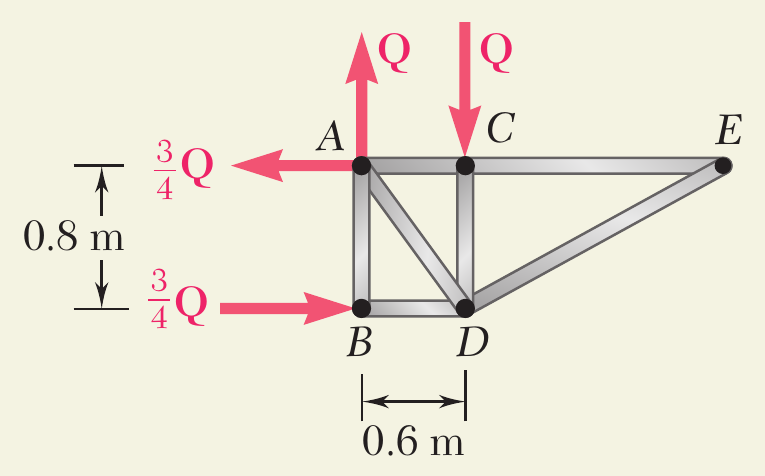
\includegraphics[width=\linewidth,height=1.9cm,keepaspectratio]{Chap_11/sp_11_5_c.png}\\[2pt]
      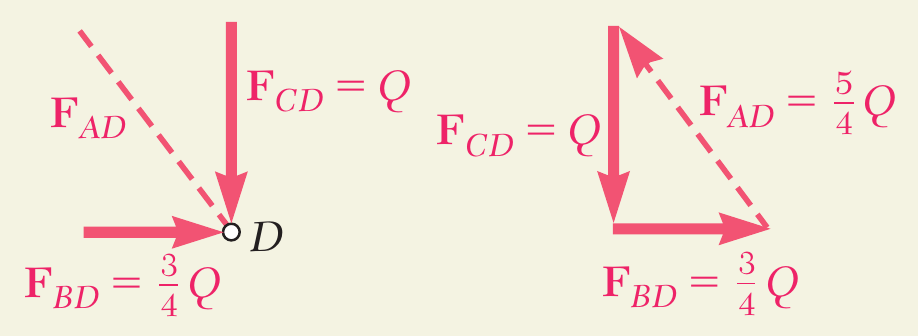
\includegraphics[width=\linewidth,height=1.9cm,keepaspectratio]{Chap_11/sp_11_5_d.png}
  \end{columns}
\end{frame}
% ===========
\begin{frame}[t]{Bài mẫu 11.5 (tiếp)}
  \begin{columns}[T]
    \column{0.58\textwidth}
      \small
      \begin{itemize}
        \setlength{\itemsep}{0.6em}
        \item Kết hợp với kết quả Bài mẫu 11.4 để tính đạo hàm theo $Q$ của năng
              lượng biến dạng của giàn do các tải trọng $P$ và $Q$:
        \[
          y_C = \sum\left(\frac{F_iL_i}{A_iE}\right)\frac{\partial F_i}{\partial Q}
            = \frac{1}{E}\left(4306P + 4263Q\right)
        \]
        \item Cho $Q = 0$, tính giá trị đạo hàm, chính là chuyển vị cần tìm tại
              $C$:
        \[
          y_C = \frac{4306(40\times10^{3}\,\mathrm{N})}{73\times10^{9}\,\mathrm{Pa}}
          \qquad \boxed{y_C = 2{,}36\,\mathrm{mm}\downarrow}
        \]
      \end{itemize}
    \column{0.40\textwidth}
      \centering
      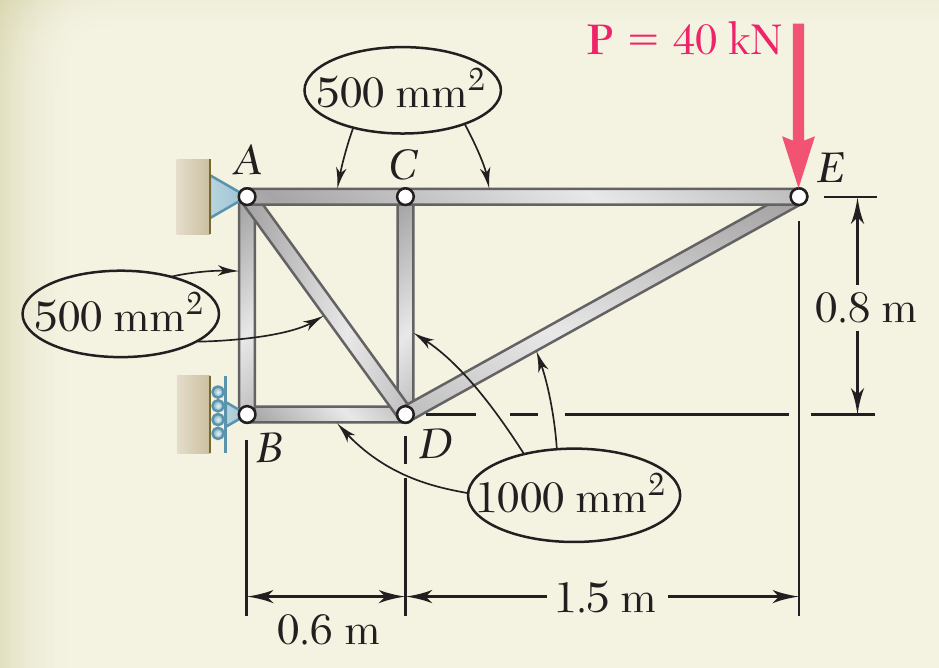
\includegraphics[width=\linewidth,height=5.5cm,keepaspectratio]{Chap_11/sp_11_5_a.png}
  \end{columns}
\end{frame}

\end{document}
